%!TEX root = ULL_thesis_template.tex 
\chapter{Learning Efficient Jumping Strategies for the Monopode System}
\label{chapter2}

% \section{Learning Control Strategies}

Utilizing reinforcement learning to train a neural network based controller has been shown to be useful for controlling many robotic systems \cite{Vecerik2017, Plappert2018}. It has been used to successfully control rigid-legged robots both in simulation and on physical hardware \cite{Ha2020a, Zhao2020}. Reinforcement learning has been shown to be capable of defining more effective and efficient-jumping techniques for a single-legged robot with SEAs \cite{Fankhauser2013}. It has also been shown to be an effective method for controlling multi-legged robots both in simulation and on physical hardware \cite{Xiao2019, Haarnoja2019a, Tsounis2019}. Furthermore, it has been shown to be useful for defining energy efficient strategies for multi-legged robots that have been deployed on physical hardware \cite{Da2020c}. However, the body of work demonstrating the use of RL to train controllers for flexible systems is limited, particularly in regards to legged locomotive systems. In this chapter, RL is deployed to define an energy efficient-jumping strategy for a monopode jumping system. The purpose of this work is to validate the use of RL for defining the control aspect of a concurrent design architecture for flexible jumping systems.

\section{Monopode Jumping System}
\label{sec:monopode}
To evaluate the methods discussed in this chapter, a monopode system like the one shown in Figure~\ref{fig:monopode} was used to represent a flexible jumping system. This system has been studied and has been shown to be an effective base for modeling the jumping gaits for many different animals \cite{Blickhan1993a}.

\begin{figure}[tb!]
    \centering
      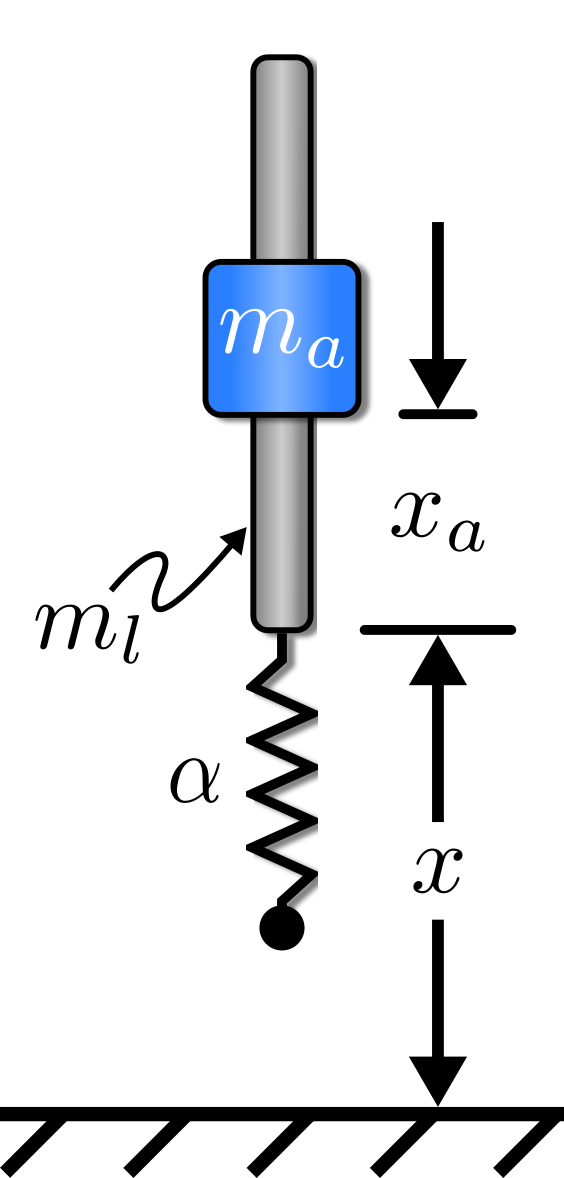
\includegraphics[width=0.25\textwidth]{Figures/Ch1/monoped.png}
      \caption{Monopode Jumping System}
      \label{fig:monopode}
\end{figure}
% 

The monopode is controlled by accelerating the actuator mass, $m_a$, along the rod mass, $m_l$, causing a hopping-like motion. The system contacts the ground through a nonlinear spring, represented by the variable $\alpha$ in the figure. Also included in the model is a damper parallel with the spring, having a damping coefficient of $c$, though it is not shown in the figure. Variables $x$ and $x_a$ represent the global position of the rod and the local position of the actuator with respect to the rod, respectively. The equation of motion for the system is: 
% 
\begin{equation}
    \label{eq:eom}
    \begin{aligned}
        \ddot{x} = \frac{\gamma}{m_t} \left(\alpha\,x + \beta\,x^3 + c\,\dot{x}\right)-\frac{m_a}{m_t}\,\ddot{x}_a-g 
    \end{aligned}
\end{equation}
%
where $x$ and $\dot{x}$ are position and velocity of the rod, respectively, the acceleration of the actuator, $\ddot{x}_a$, is the control input, and $m_a$ and $m_t$ are the mass of the actuator and the complete system, respectively. Constants $\alpha$ and $c$ represent the nonlinear spring and damping coefficient, respectively, and constant $\beta$ is set to $1e8$. Ground contact determines the value of $\gamma$, so that the spring and damper do not apply any force while the leg is airborne:
% 
\begin{equation}
    \label{eq:gamaa}
    \gamma =
    \left\{\begin{matrix}
        -1, & x \leq 0\\ 
        \hphantom{-} 0, & \mbox{otherwise}
    \end{matrix}\right.
\end{equation}  
% 
Additionally, the spring compression limit, or the systems position in the negative $x$ direction, is limited to 0.008m. The system is also confined to move only vertically so that controlling balance is not required. The values of the parameters shown in Figure~\ref{fig:monopode} are displayed in Table~\ref{tab:monopode_params}. 
% 
\begin{table}[tb!]
  \caption{Monopode Model Parameters}
    \begin{center}
    \vspace{-12pt}
      \begin{tabular}{c c}
        \textbf{Model Parameter}                                 & \textbf{Value}                                    \\
        \hline
        \hline
        Mass of Leg, $m_l$                                       & 0.175 kg                                          \\
        Mass of Actuator, $m_a$                                  & 1.003 kg                                          \\
        Spring Constant, $\alpha_{nominal}$                      & 5760 $\textup{N}/\textup{m}$                      \\
        Natural Frequency, $\omega_n$                            & $\sqrt{\frac{\alpha}{m_l + m_a}}$                 \\
        Damping Ratio, $\zeta_{nominal}$                         & 1e-2 $\frac{\textup{N}}{\textup{m/s}}$            \\
        Gravity, $g$                                             & 9.81 m/s$^2$                                      \\
        \hline
        Actuator Stroke, $(x_{a})_{\textup{max}}$                & 0.008 $\textup{m}$                                \\
        Max.\ Actuator Velocity, $(\dot{x}_{a})_{\textup{max}}$  & 1.0 $\textup{m}/\textup{s}$                       \\ 
        Max.\ Actuator Acceleration, $(\ddot{x}_{a})_{\textup{max}}$   & 10.0 $\textup{m}/\textup{s}^2$              \\
        \hline
        \hline
      \end{tabular}
      \label{tab:monopode_params}
      % \vspace{-12pt}
    \end{center}
\end{table}
%  

\section{Training Environment}
Using the monopode model, an environment aligning with the standards set by OpenAI for a Gym environment was created \cite{Brockman2016c}. The observation and action spaces were defined, respectively, as follows:
% 
\begin{equation}
  \mathcal{S} = \left[ x_{a_t}, \dot{x}_{a_t}, x_t, \dot{x}_t \right]
\end{equation}
% 
\begin{equation}
  \mathcal{A} = [\ddot{x}_{a_t}]
\end{equation}
% 
where $x_t$ and $\dot{x}_t$ were the monopode's position and velocity at time $t$, and $x_{a_t}$, $\dot{x}_{a_t}$ and $\ddot{x}_{a_t}$ were the actuator's position, velocity and acceleration, respectively.

Two separate stopping conditions were defined for the environment to evaluate two different jump types and therefore two different jumping commands. The first was defined as the position of the monopode being greater than zero then returning to zero once. The second condition was defined like the first condition, but with the position of the monopode being greater than zero and then returning than zero twice.

Two different jumps were created from these stopping conditions. The first was a single jump command, and the second a stutter jump command. The intent of utilizing two different jumping commands was to determine if an RL algorithm was more or less effective in learning differing strategies depending on the complexity of the desired command. 

% 
\begin{figure}[tb!]
  \centering
  \begin{subfigure}{.75\textwidth}
    \centering
    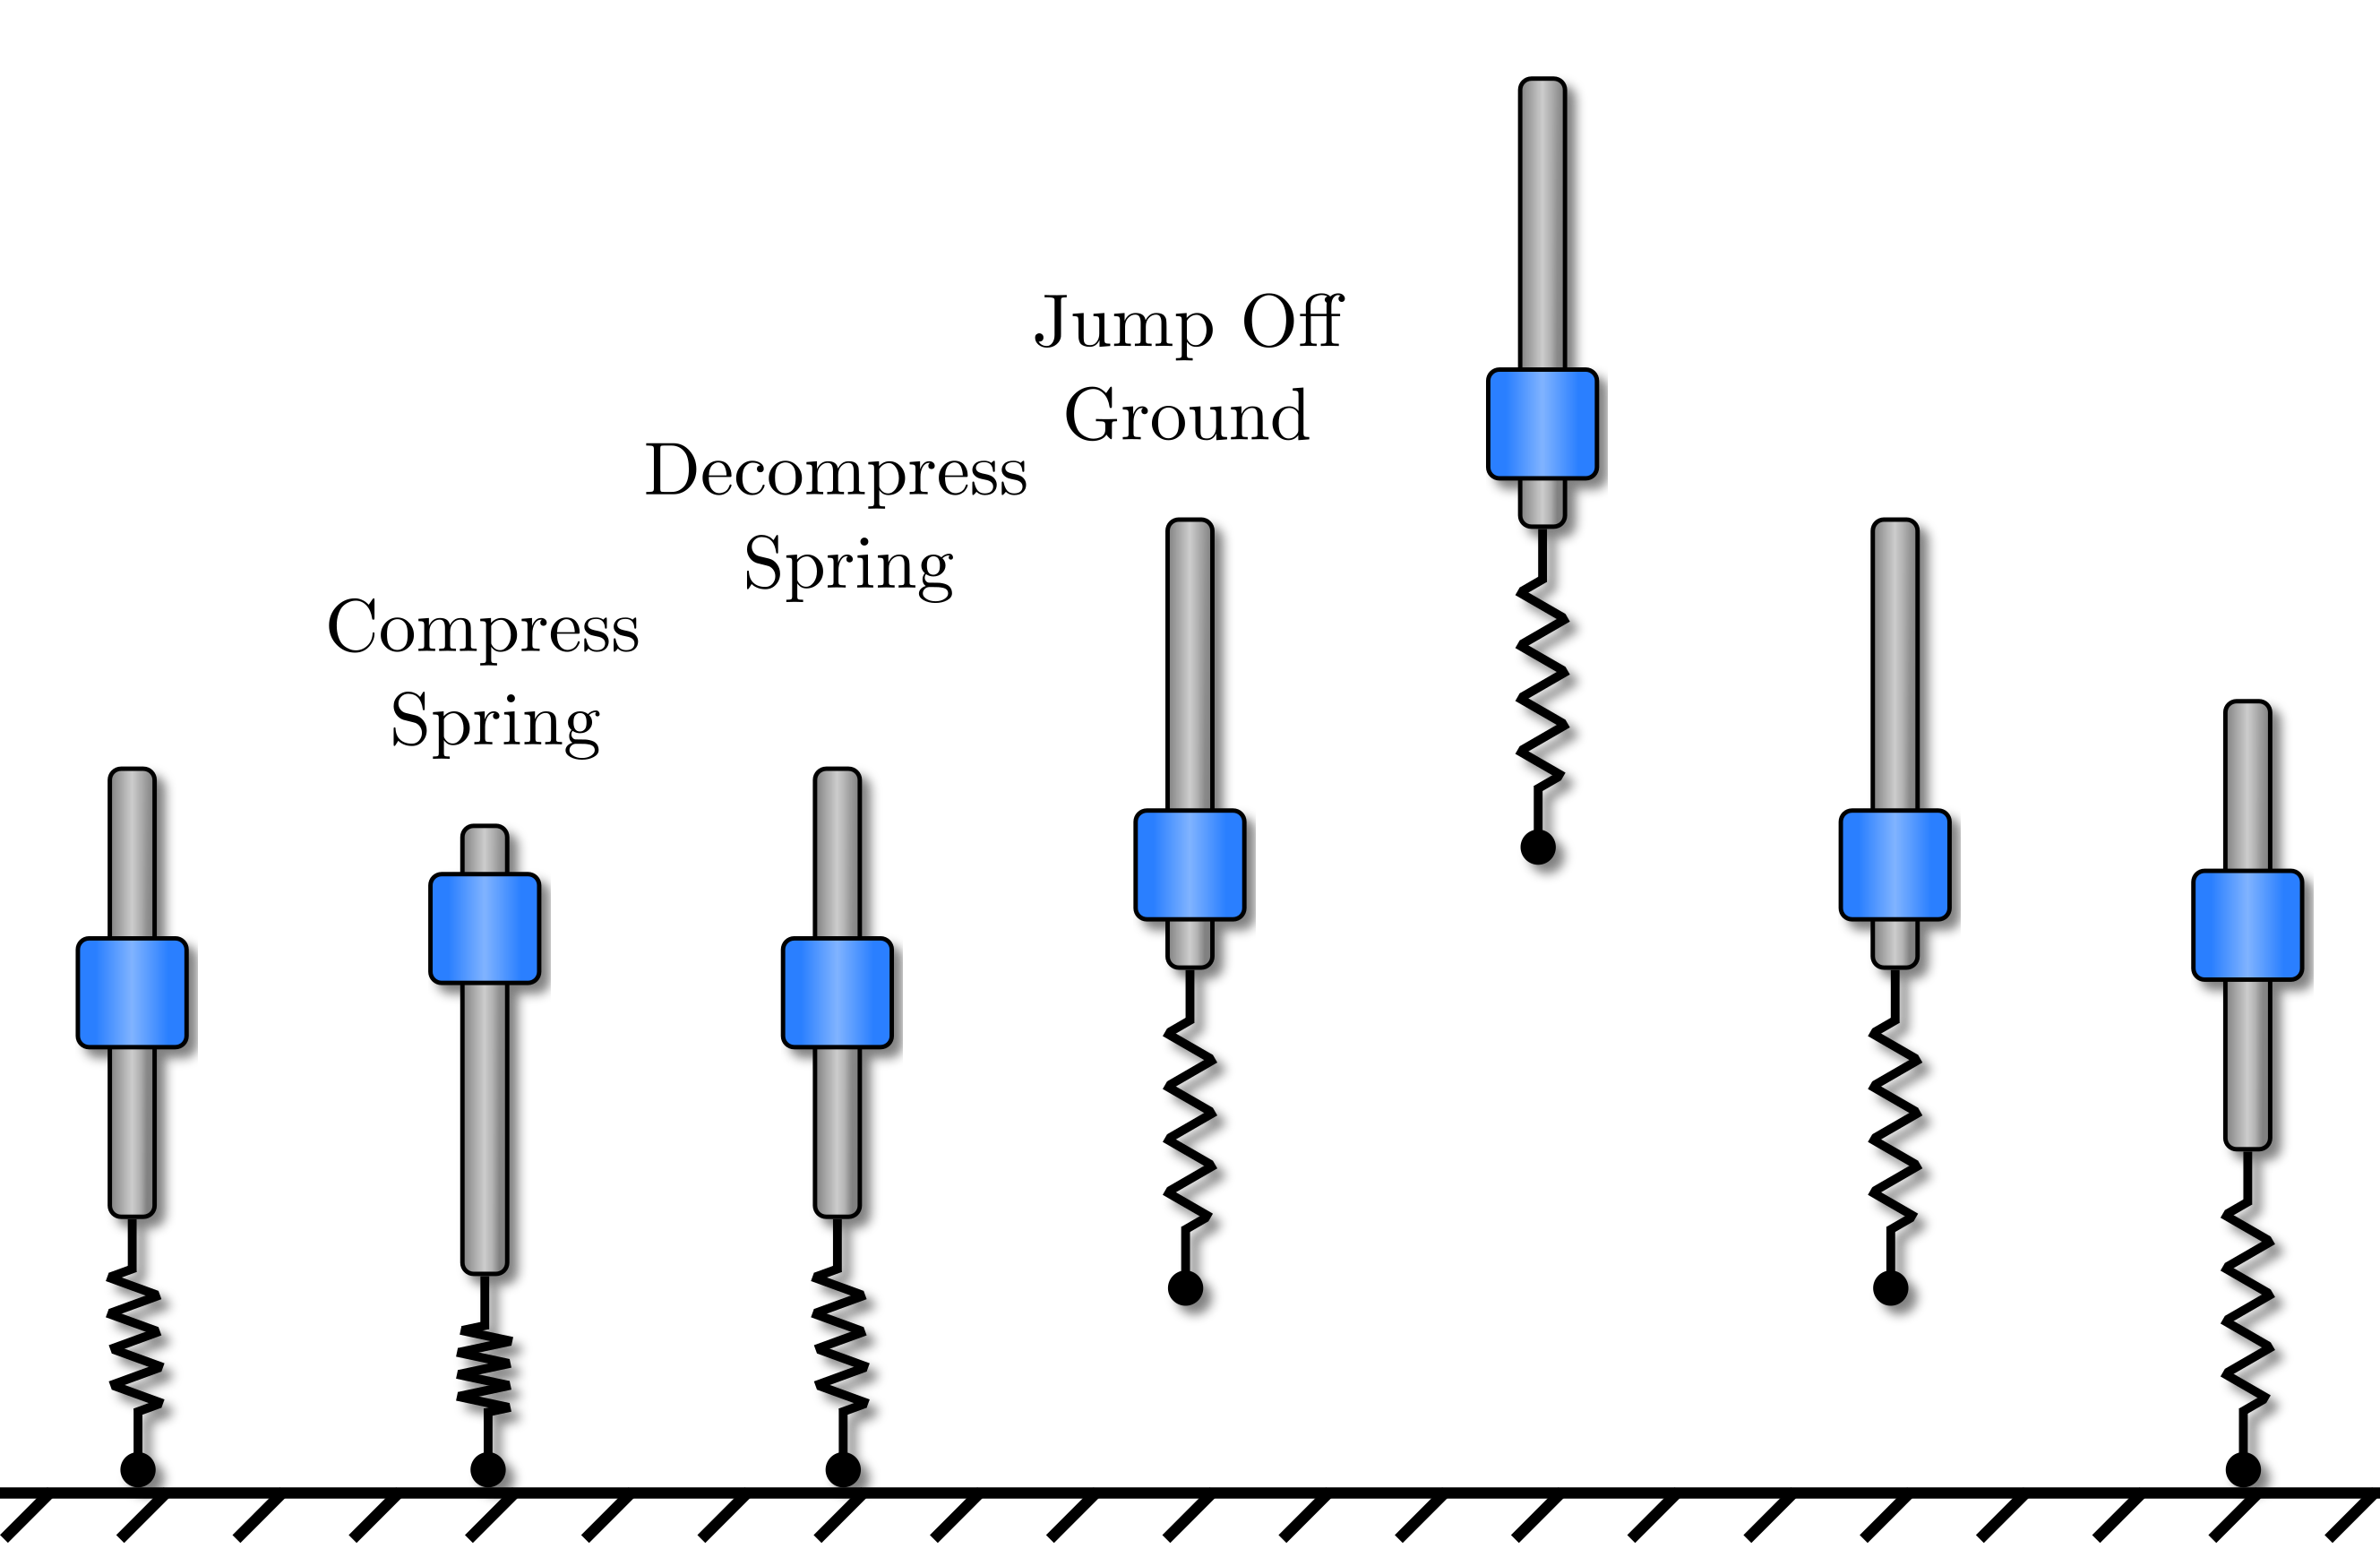
\includegraphics[width=\linewidth]{Figures/Ch2/single_jump.png}
    \caption{Example Single Jump}
    \label{fig:singleJump}
  \end{subfigure} \\
  \begin{subfigure}{.9\textwidth}
    \centering
    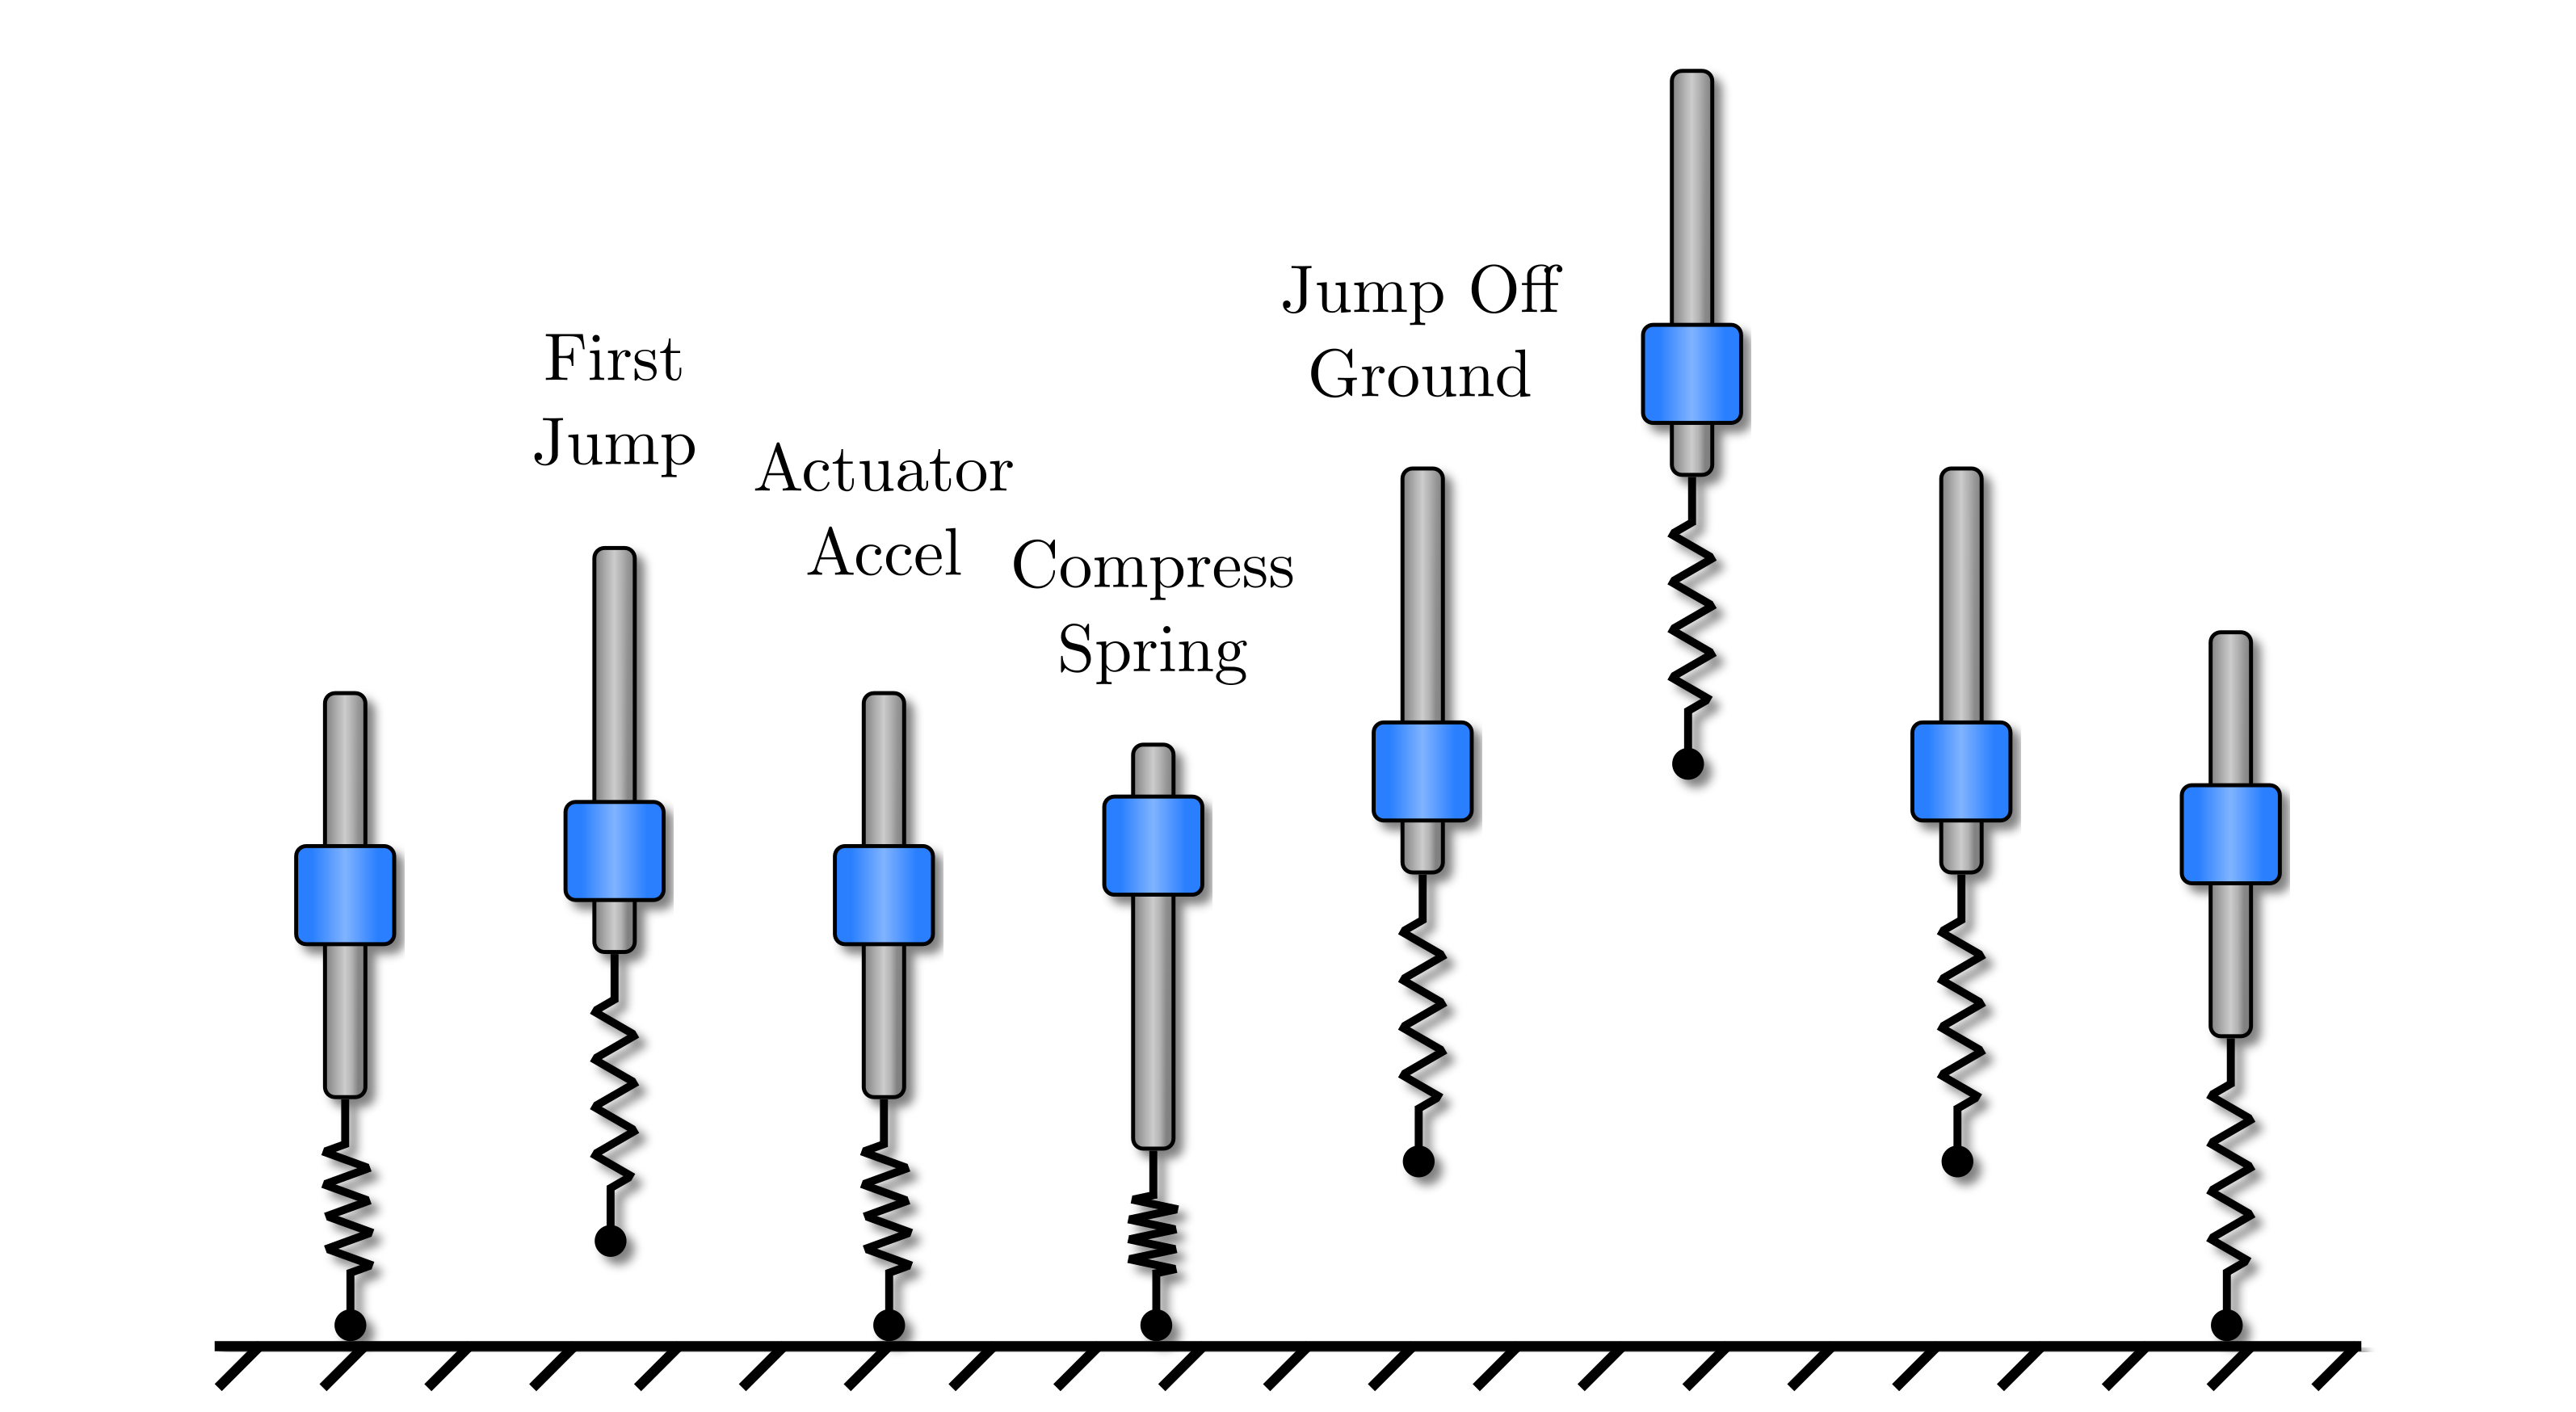
\includegraphics[width=\linewidth]{Figures/Ch2/stutter_jump.png}
     \caption{Example Stutter Jump}
     \label{fig:stutterJump}
  \end{subfigure}
   \caption{Jumping Types for the Monopode Jumping System}
   \label{fig:jump_types}
\end{figure} 

An example single jump is shown in Figure~\ref{fig:singleJump}. The intended command from the learned controller would be one that would jump the monopode once. This type of command would ideally compress the spring/damper by accelerating the actuator in the positive direction. This would cause the rod mass to accelerate downward compressing the spring to store energy that could be used to cause the system to jump. The actuator mass should then accelerate downward forcing the spring to decompress. At this point, the system should be accelerating upwards and the actuator downwards such that the monopode leaves the ground completing a single jump. 

An example stutter jump can be seen in Figure~\ref{fig:stutterJump}. The intended command from the learned controller would be one that would jump the monopode twice. This type of command would firstly complete an optimal single jump. Following that motion, the actuator should accelerate to recompress the spring, storing more energy with a farther compression. When the spring is compressed to its maximum value or the total acceleration of the system reaches zero, the actuator mass should accelerate downwards forcing the spring to decompress. At this point, the system should be accelerating upwards and the actuator downwards, similar to the single jump, such that the monopode leaves the ground completing a stutter jump.

\section{Efficient Control Strategies}
% 
Efficient control of a robotic system is often one of the most important aspects of a given controller design. Applications where a robotic system is deployed and relies on a limited power source, such as a mobile walking robot, will often require an efficient control strategy. Modern, traditional methods, such as model predictive control, have been shown to produce energy efficient locomotion strategies for wheeled and legged systems \cite{Harper2019, Pace2017}. In this work, a modern neural network based control method utilizing RL techniques is used to find strategies that are designed with power efficiency as the primary objective.

Two different reward functions were designed to accomplish the task of determining how well RL learns efficient-jumping strategies. The purpose of defining two different reward functions was to compare the commands and resulting jumping performance of the two controller types to determine if the efficient controller was learning to conserve power. 

The first reward function was one that ignored power usage and focused solely on the height of the jump:
% 
\begin{equation}
    \label{eq:rewardHeight}
    R = x_t
\end{equation}
% 
where $x_t$ was the height of the monopode system at any given time step. The second reward function was one that was defined to accomplish the same task, but also consider power consumption. It was defined as:
% 
\begin{equation}
    \label{eq:rewardEfficiency}
    R = \frac{x_t}{\sum_{t=0}^{t} P_t}
\end{equation}
% 
where $P_t$ was the power consumption of the monopode system at any given time step defined mechanically as the product of the actuator's acceleration, velocity, and mass:
%
\begin{equation}
    \label{eq:power}
    P_t = m_a\,\dot{x}_a\,\ddot{x}_a
\end{equation}
%
where $m_a$ was the mass of the actuator, and $\dot{x}_a$ and $\ddot{x}_a$ where the actuators velocity and acceleration, respectively. 

\section{Deploying TD3}
% 
Because RL may generate a locally optimal controller instead of a globally optimal controller, training more than one controller is common practice for evaluating performance. In this work, fifty different controllers where trained, each with a different random network initialization. Each controller was trained for a total 500k time steps. The remaining hyperparameters set using the TD3 algorithm are defined in Table~\ref{tab:ctr_hyperparams}.

\begin{table}[tb!]
  \caption{TD3 Training Hyperparameters}
  \begin{center}
  \vspace{-12pt}
  \begin{tabular}{c c}
  \textbf{Hyperameter}            & \textbf{Value}                  \\
  \hline
  \hline
  Learning Rate, $\alpha$         & 0.001                           \\
  Learning Starts                 & 1000 Steps                      \\
  Batch Size                      & 100 Transitions                 \\
  Tau, $\tau$                     & 0.005                           \\
  Gamma, $\gamma$                 & 0.99                            \\
  Training Frequency              & 1:Episode                       \\
  Gradient Steps                  & $\propto$ Training Frequency    \\
  Action Noise,  $\epsilon$       & None                            \\
  Policy Delay                    & 1 : 2 Q-Function Updates        \\
  Target Policy Noise, $\epsilon$ & 0.2                             \\
  Target Policy Clip, $c$         & 0.5                             \\
  Seed                            & 50 Random Seeds                 \\
  \hline
  \hline
  \end{tabular}
  \label{tab:ctr_hyperparams}
  \end{center}
\end{table}
%
\begin{figure}[tb!]
  \centering
  \begin{subfigure}{.49\textwidth}
    \centering
    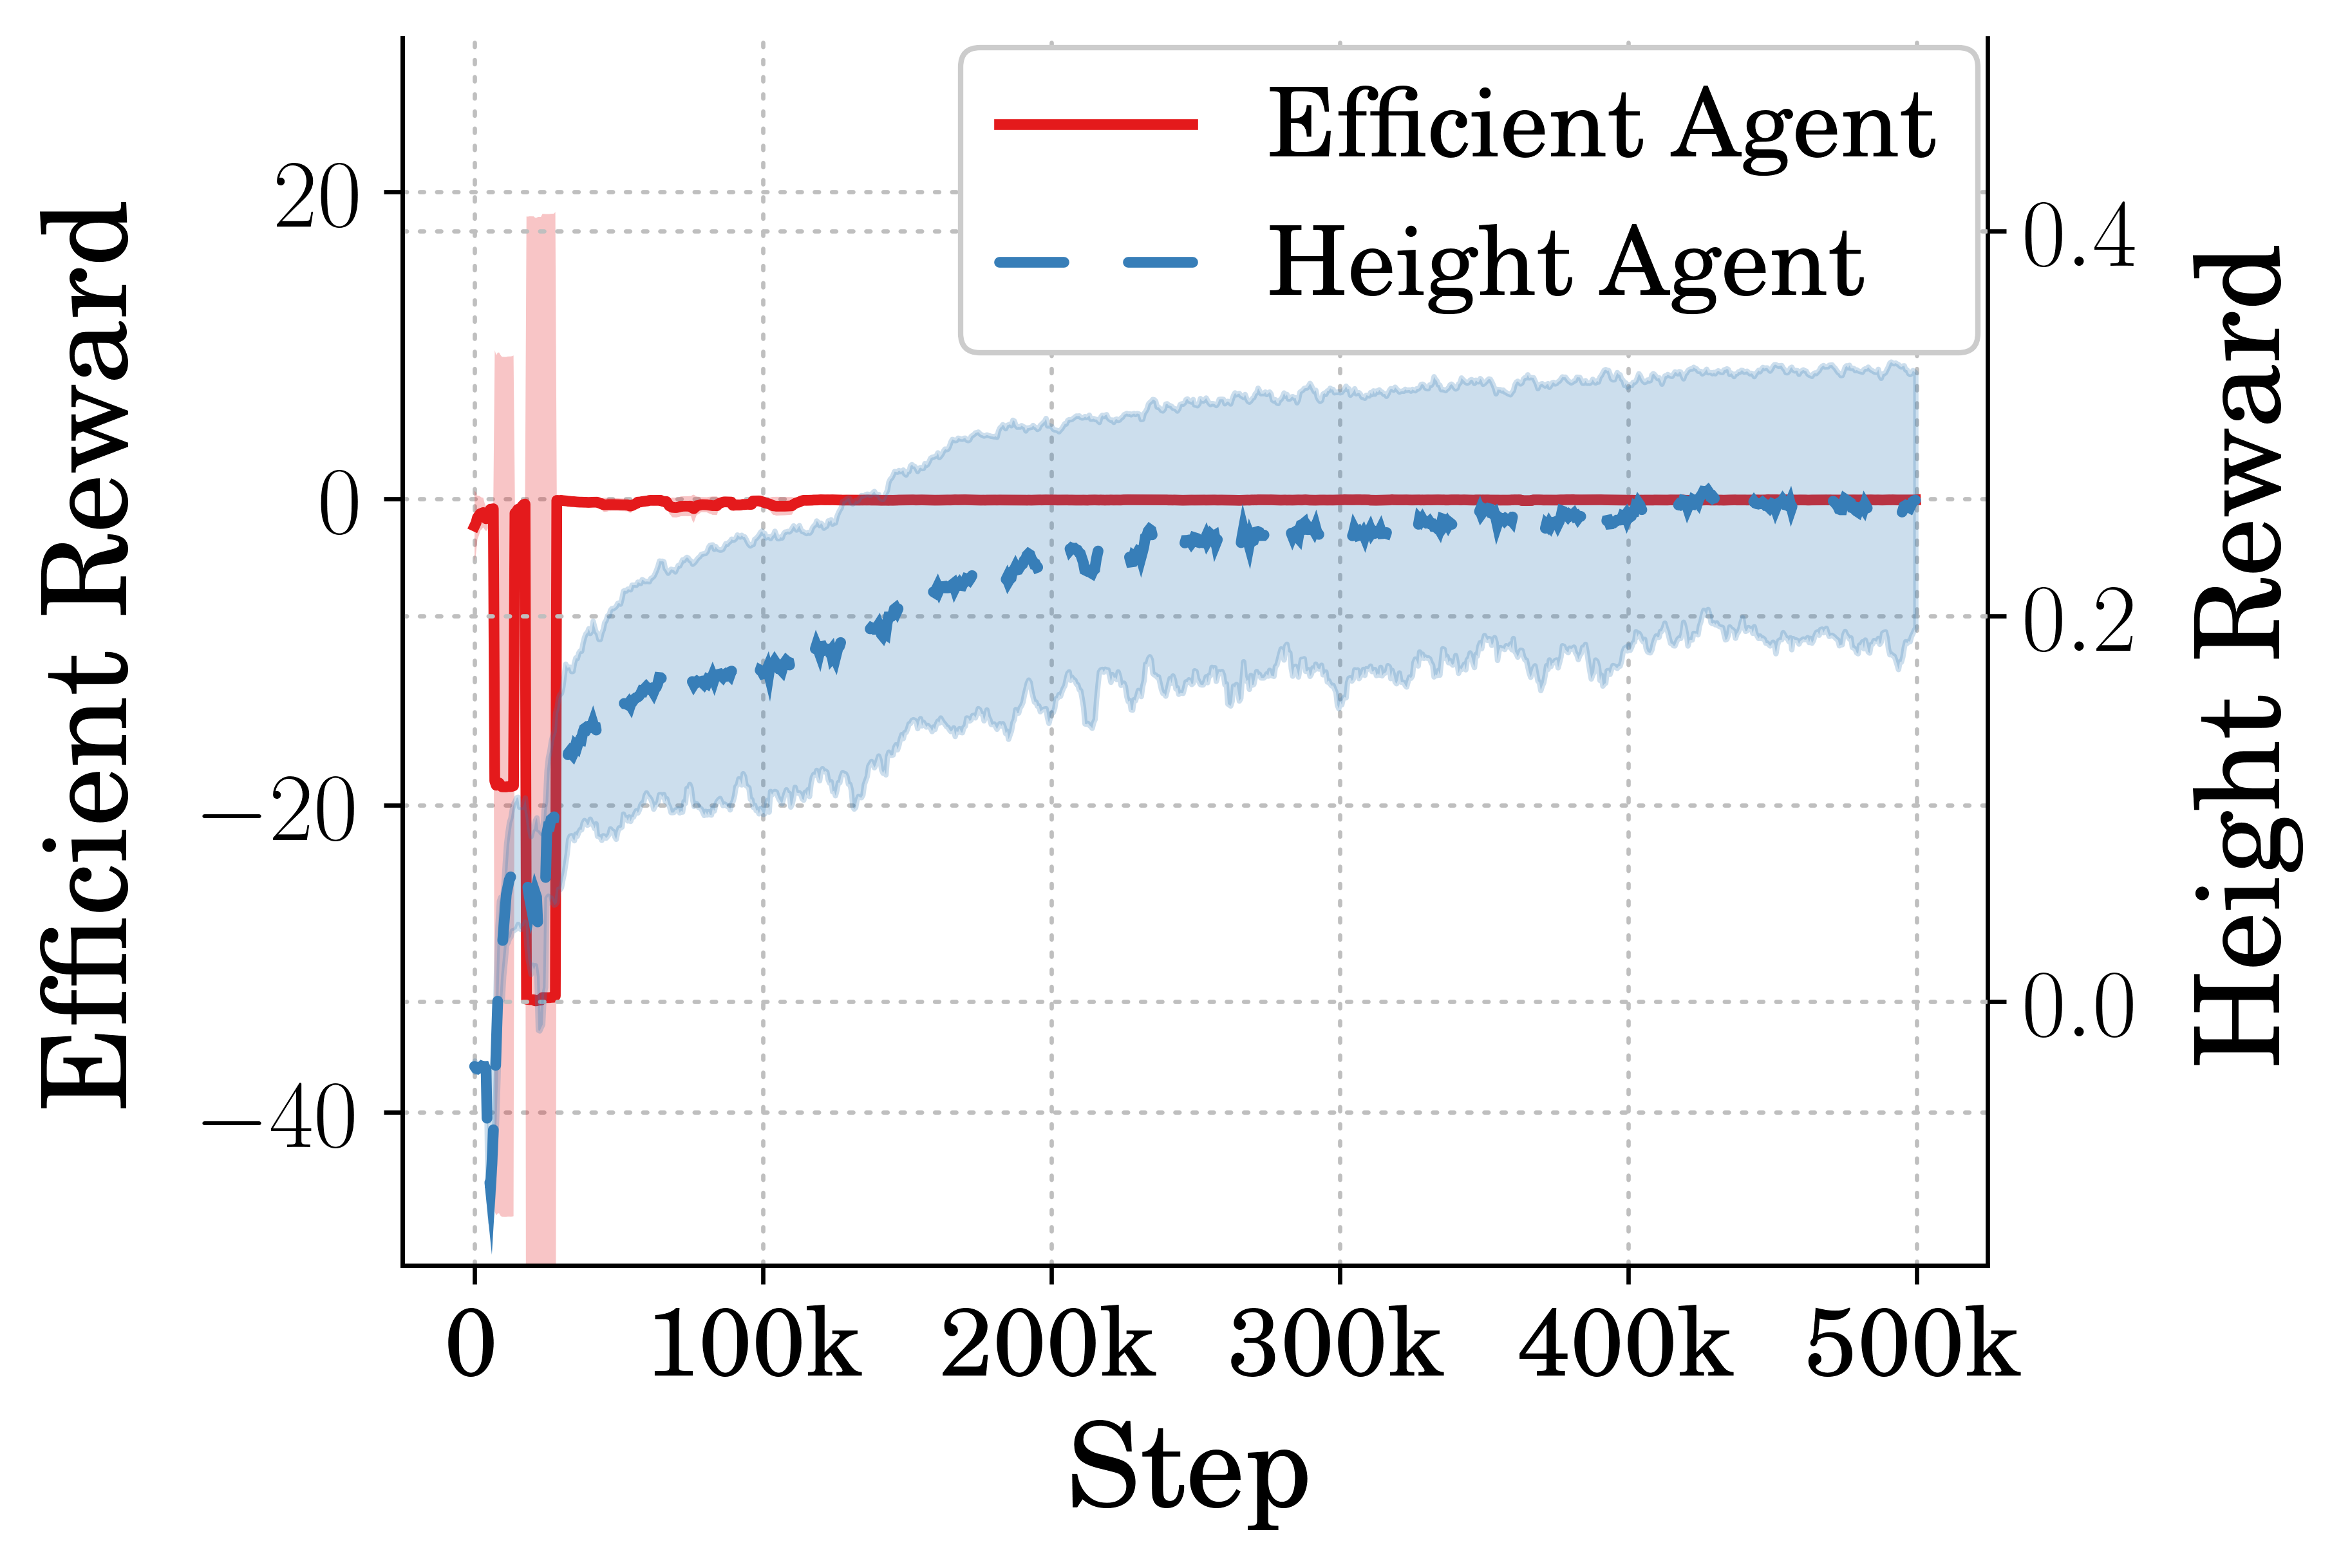
\includegraphics[width=\linewidth]{Figures/Ch2/RewVsTimeOne.png}
    \caption{Single Jumping Reward}
    \label{fig:avg_one_rew}
  \end{subfigure}%
  \hfill
  \begin{subfigure}{.49\textwidth}
    \centering
    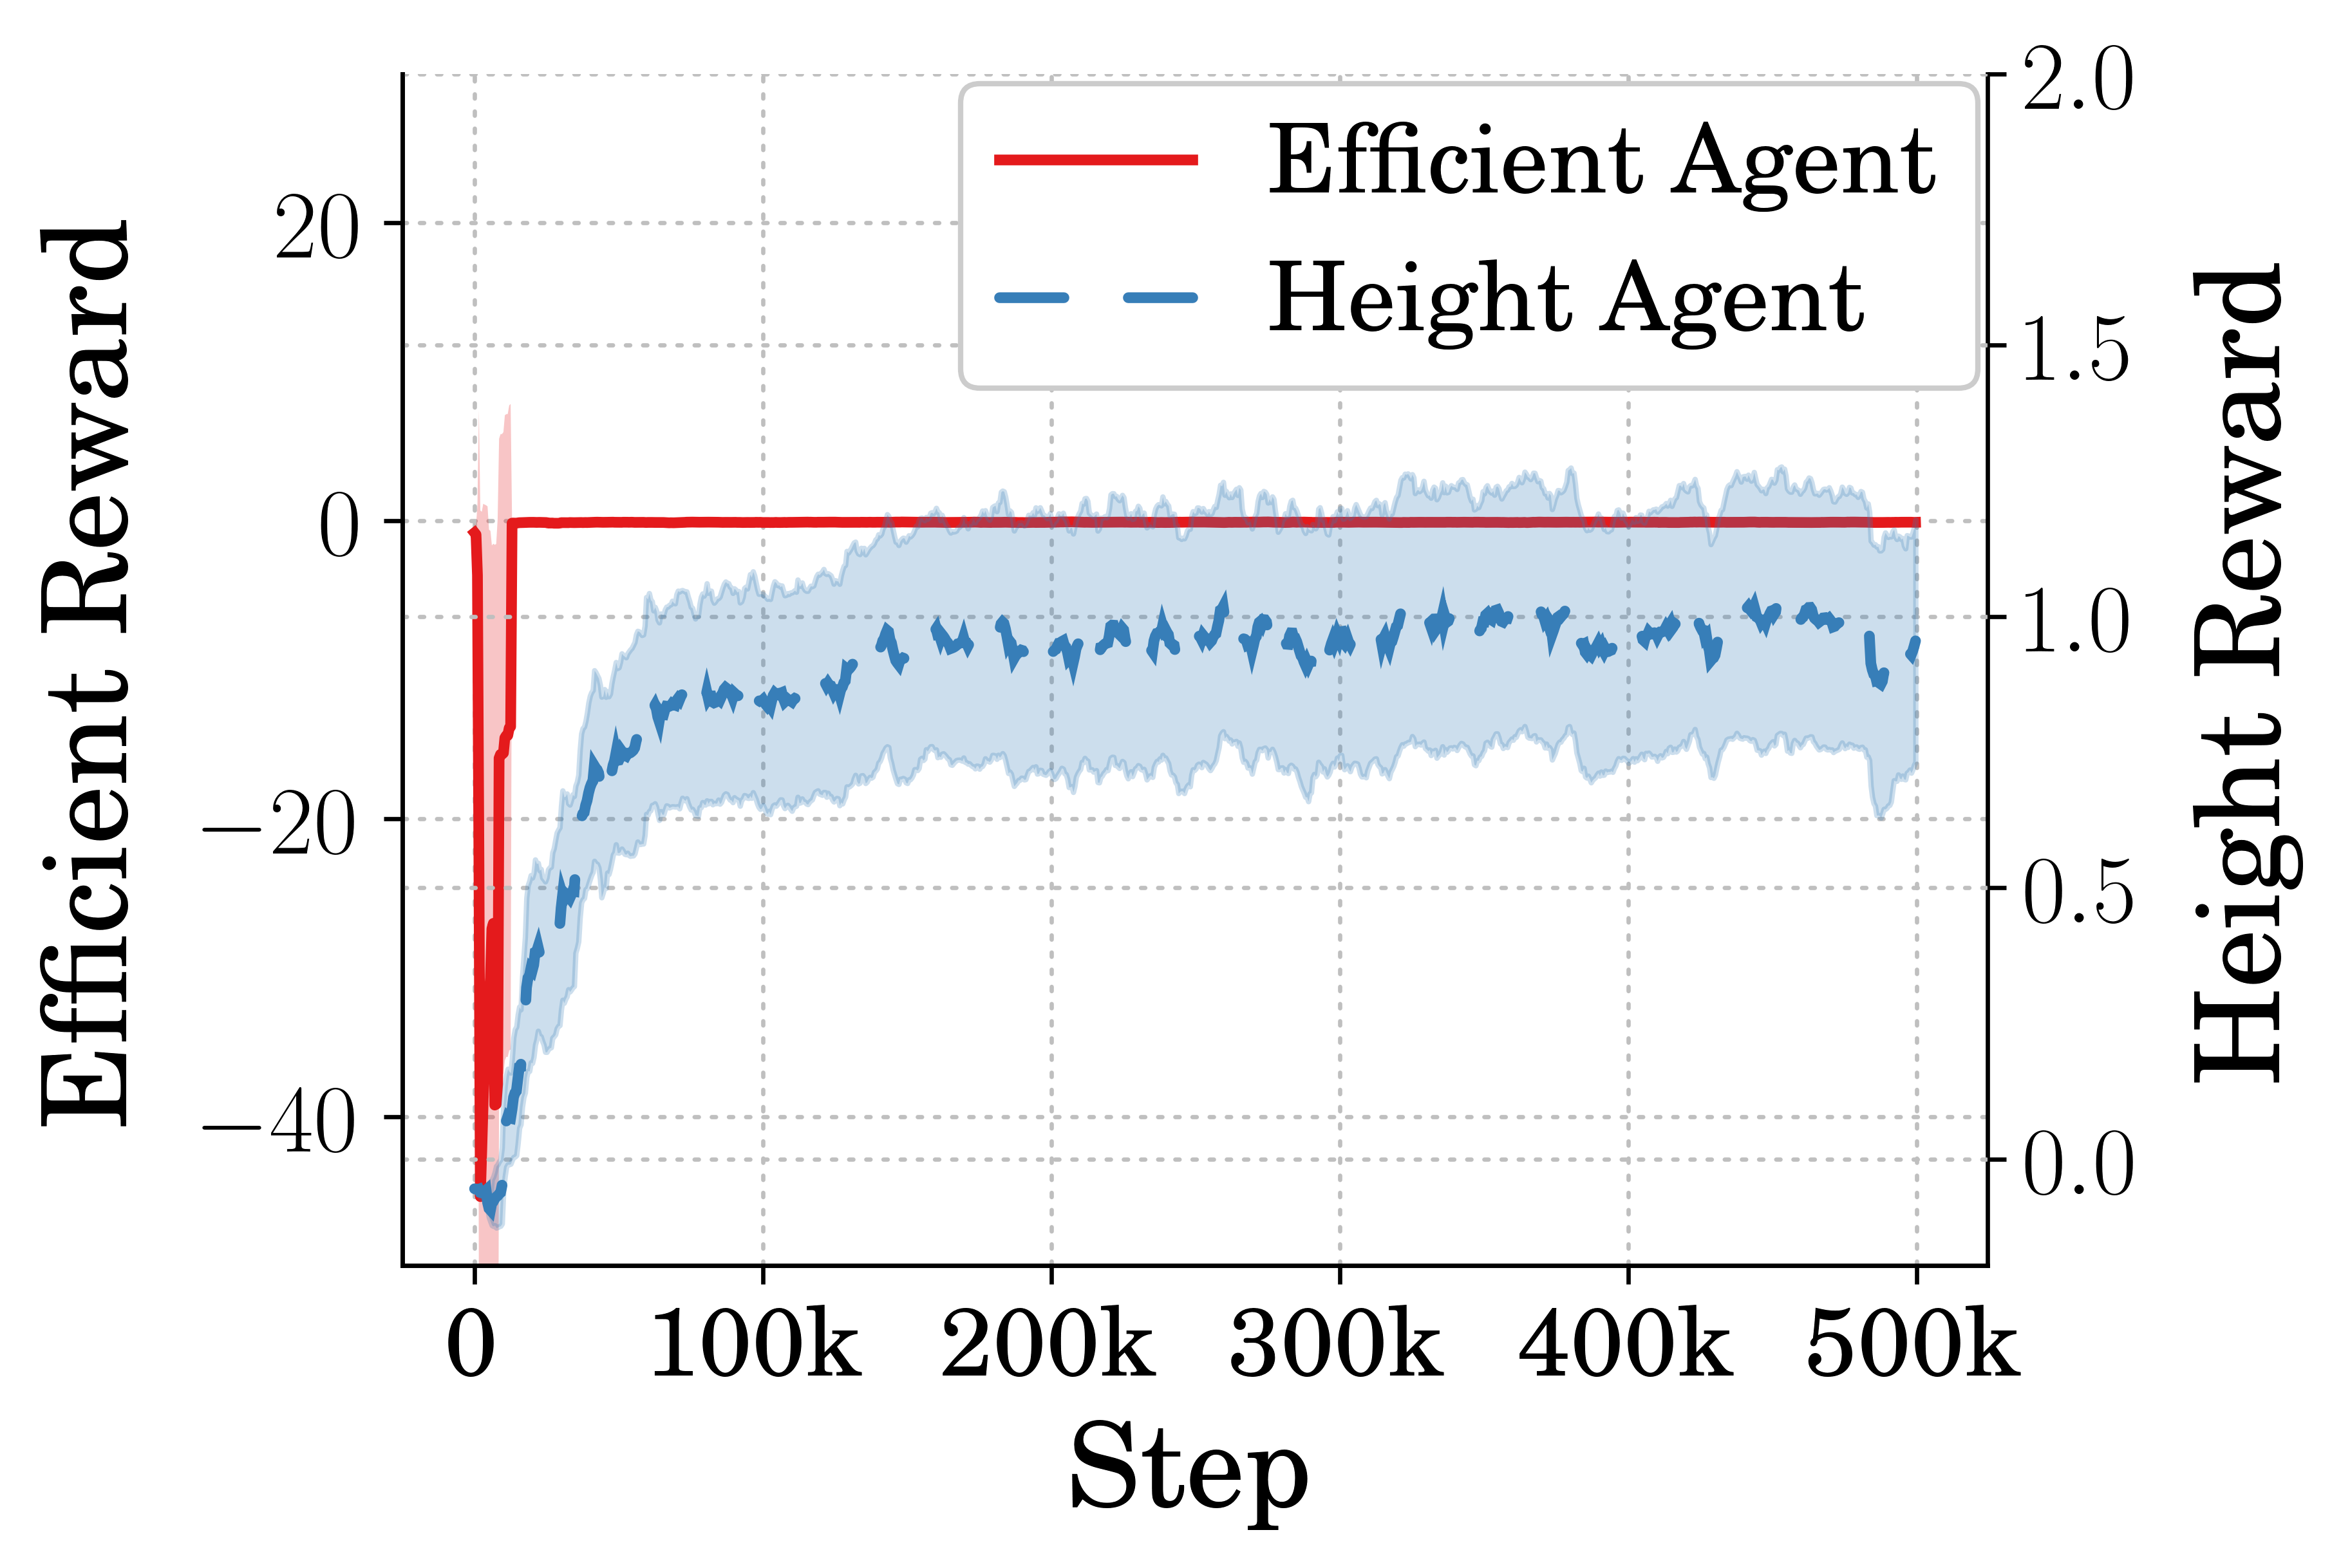
\includegraphics[width=\linewidth]{Figures/Ch2//RewVsTimeStutter.png}
     \caption{Stutter Jumping Reward}
     \label{fig:avg_stutter_rew}
  \end{subfigure}
   \caption{Reward vs Time Step During Training}
   \label{fig:avg_rew}
\end{figure}
% 

The average and standard deviation of the rewards during training for the efficient and high jumping strategies for both the single and stutter jumping commands are shown in Figure~\ref{fig:avg_rew}. They represent the controllers being trained to accomplish their respective goals. Looking at Figure~\ref{fig:avg_one_rew}, which shows the rewards for learning a single jumping command, it is clear that there are definite differences between the efficient and high-jumping reward types. Firstly, the high-jumping strategy does converge after 500k steps of training. The reward for the efficient-jumping controller, having been defined drastically different than the reward from the high-jumping controller, not surprisingly, looks drastically different than the high-jumping reward. The reward for the efficient agent is heavily punished for using power without gaining height, which is a frequent occurrence in the beginning of training. This forces the policy to learn that using less power will result in higher rewards within very few learning steps. In Figure~\ref{fig:avg_stutter_rew}, it is also apparent that the height controller converged to a solution. Additionally, the efficient controller can be seen to have learned in the same rapid form as the single jumping command type. 


\section{Average Performance of Network Controller}
\label{section:avg_performance}
% 
\subsection{Jumping commands}
\label{subsection:avg_input_performance}
% 
\begin{figure}[tb!]
  \centering
  \begin{subfigure}{.49\textwidth}
    \centering
    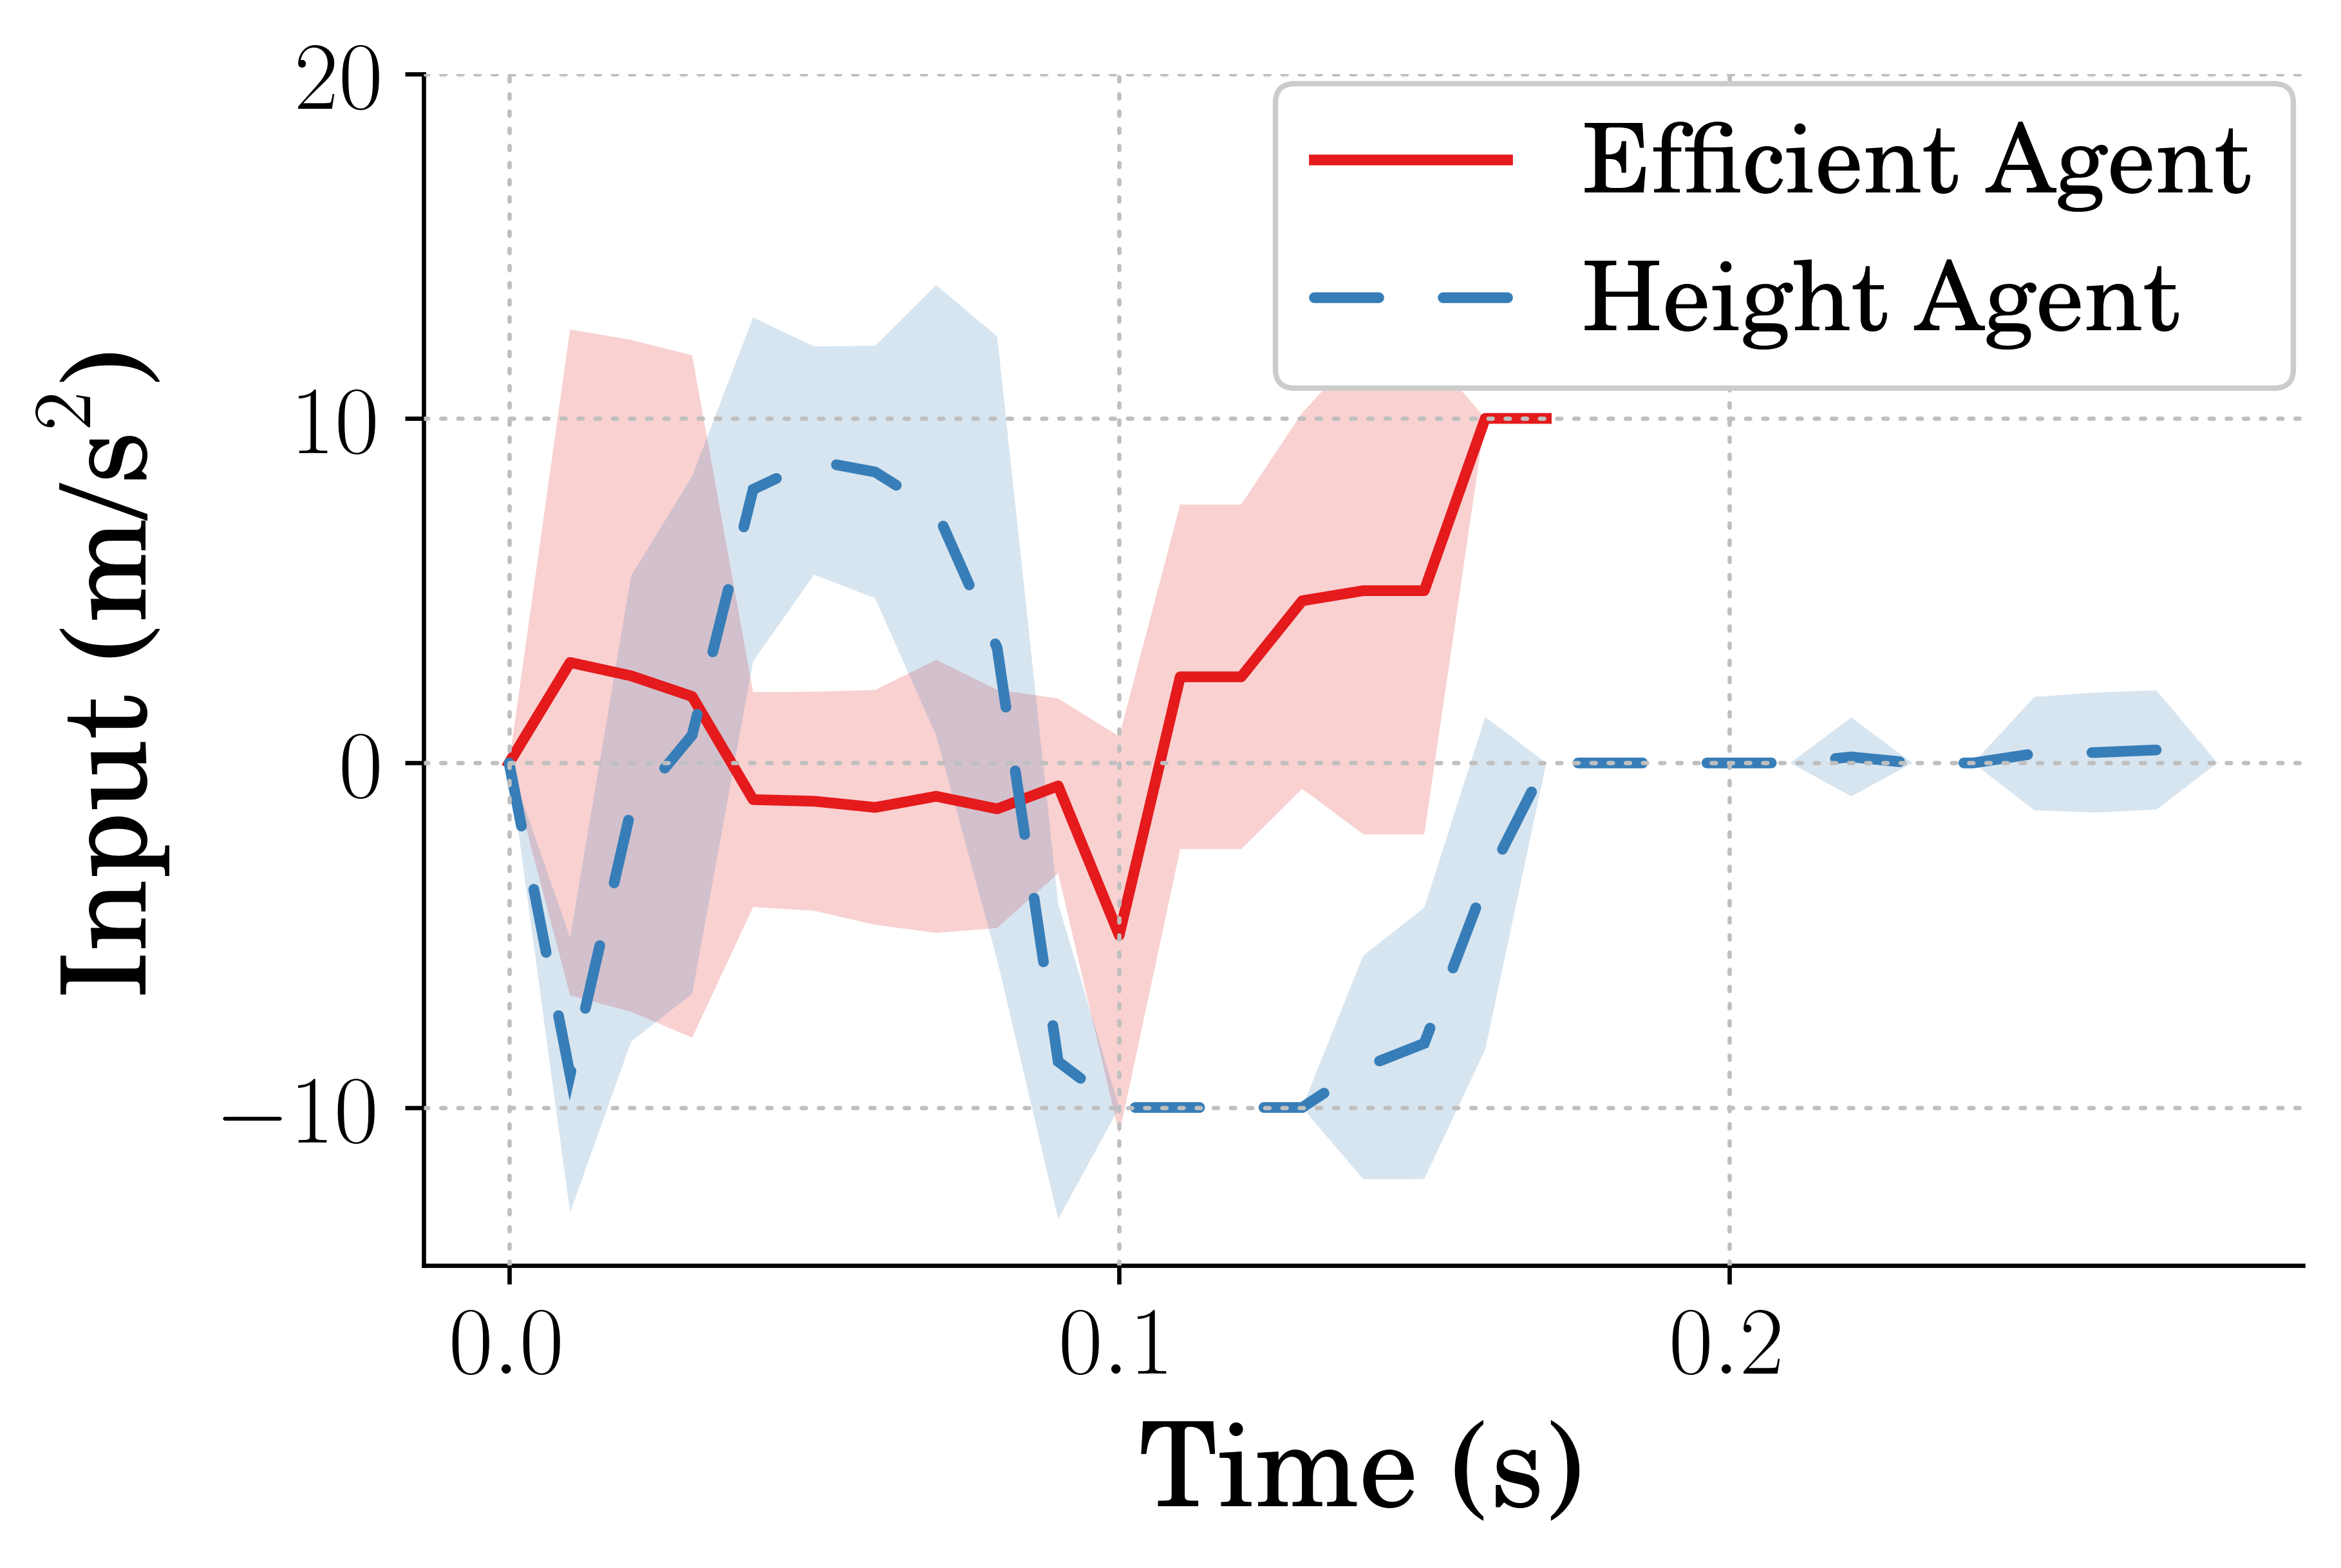
\includegraphics[width=\linewidth]{Figures/Ch2/avg_One_Input_.png}
    \caption{Single Jumping Input}
    \label{fig:avg_one_input}
  \end{subfigure}%
  \hfill
  \begin{subfigure}{.49\textwidth}
    \centering
    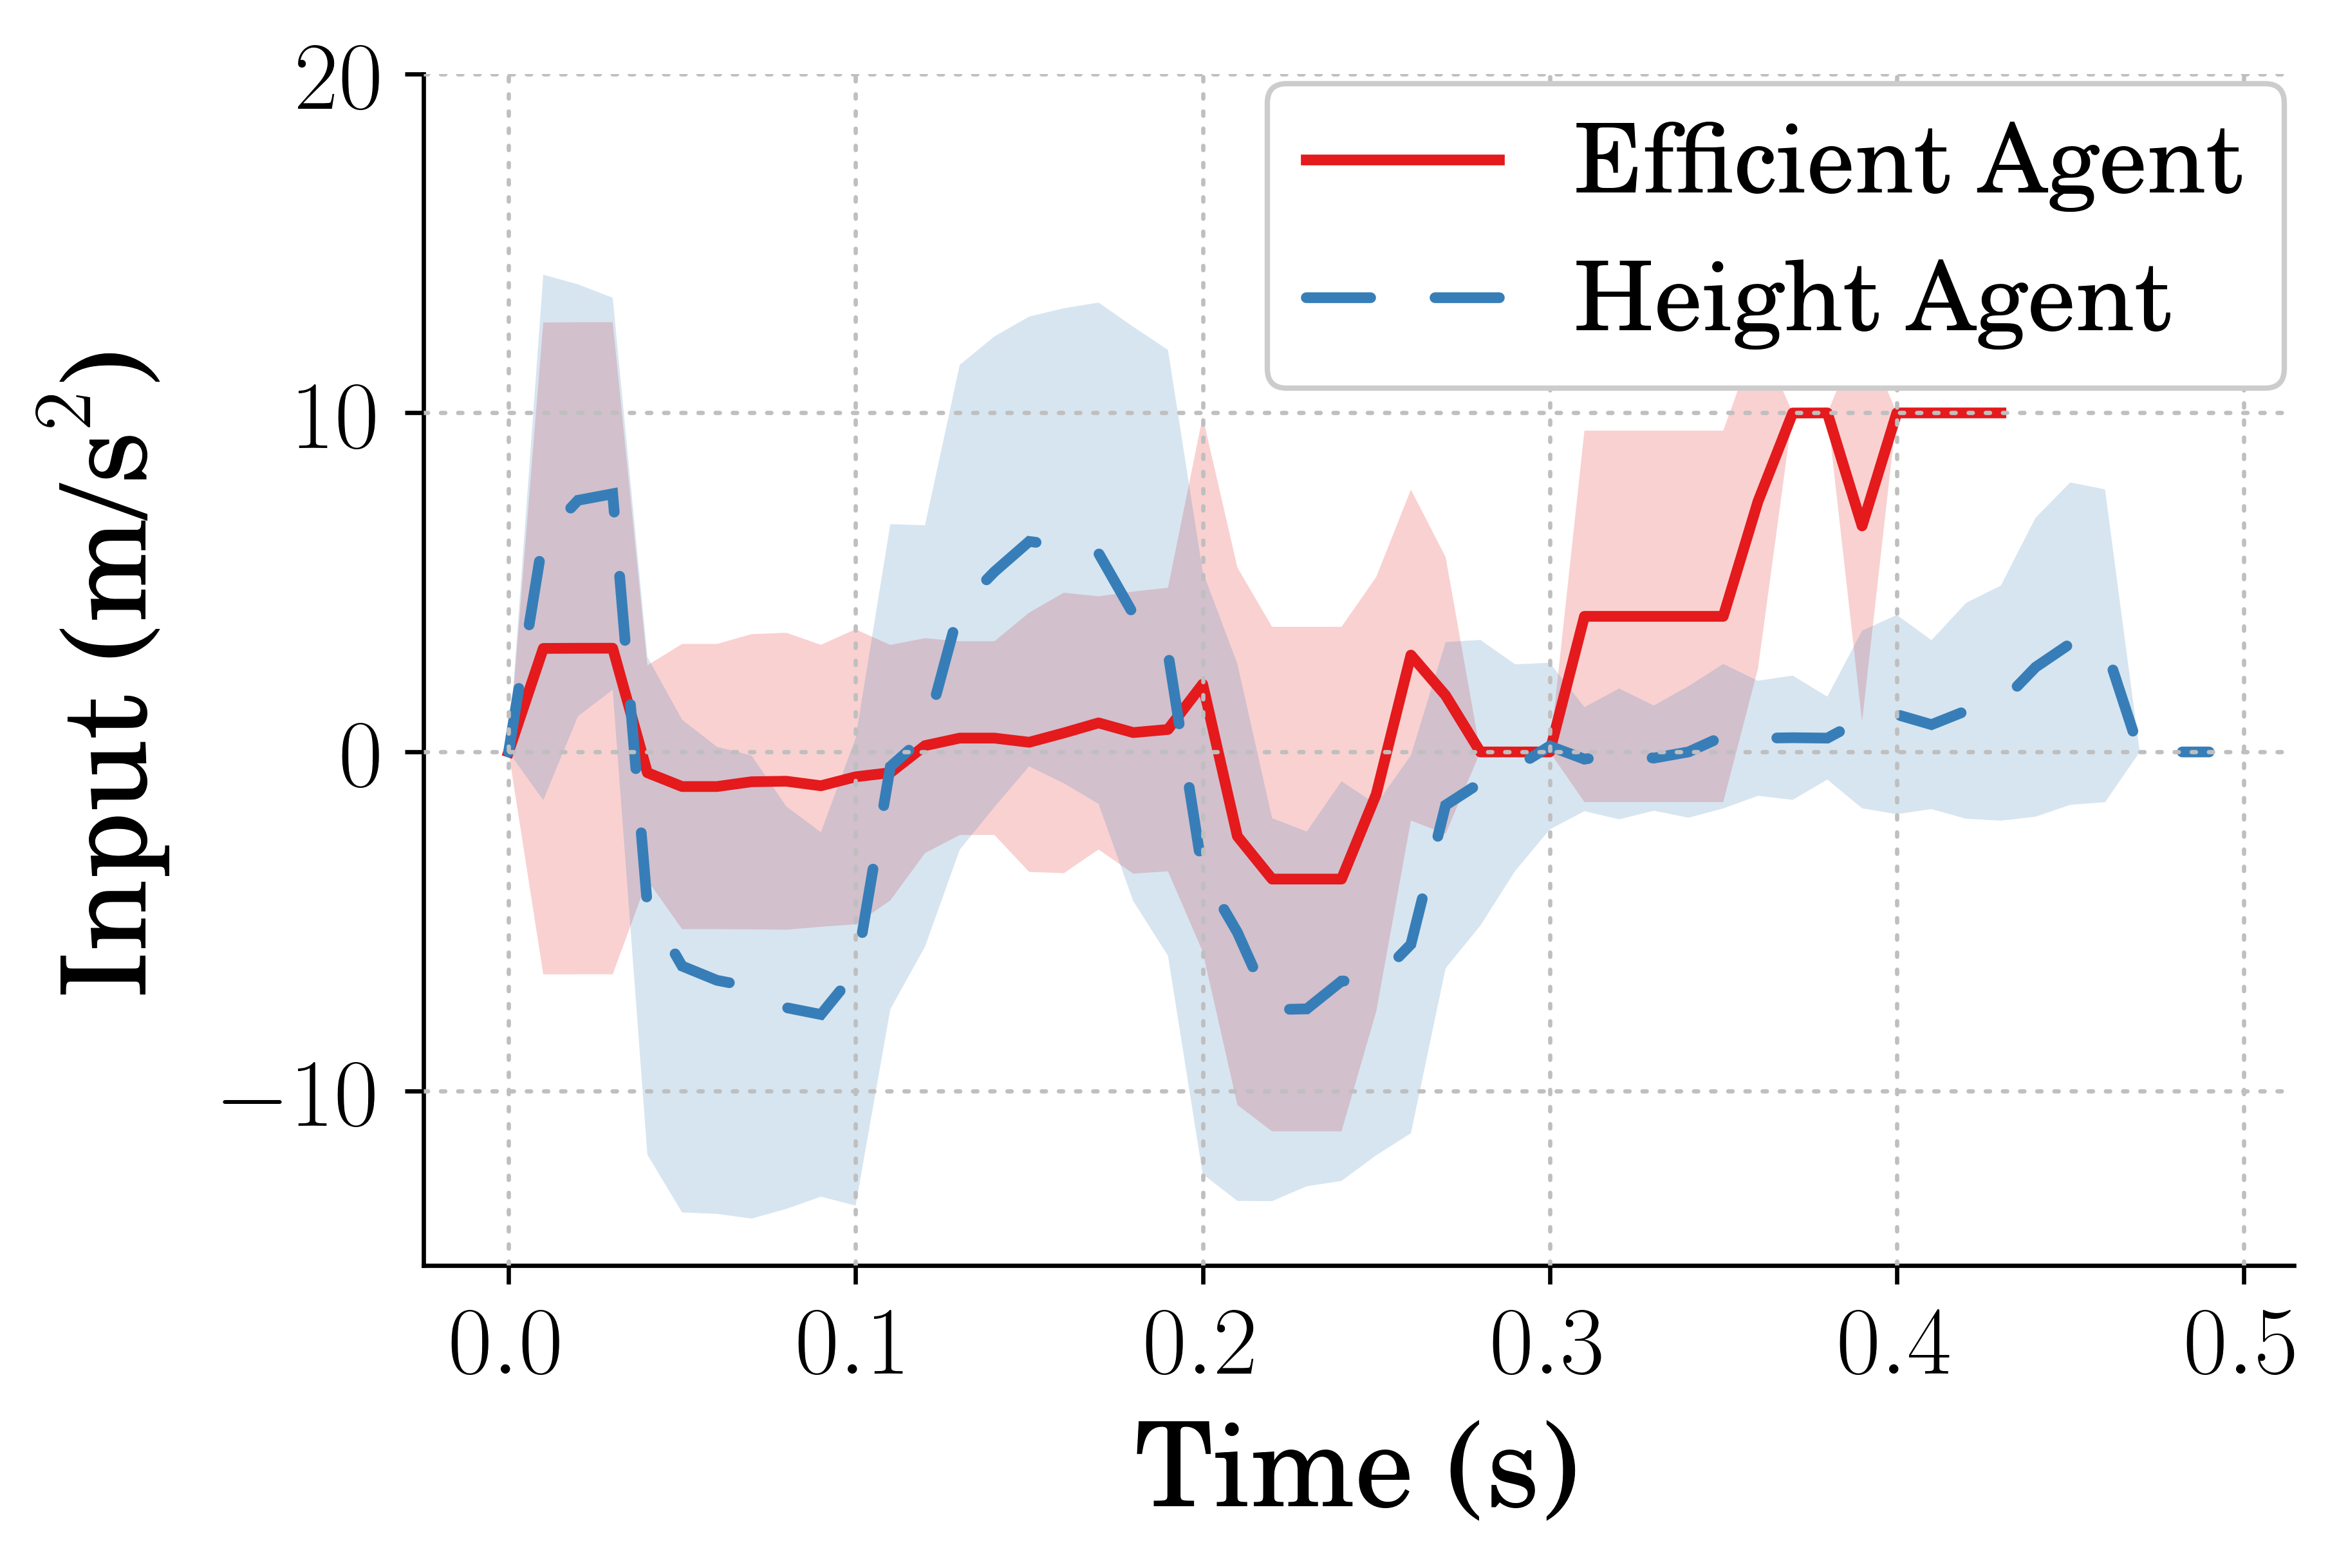
\includegraphics[width=\linewidth]{Figures/Ch2/avg_Stutter_Input_.png}
     \caption{Stutter Jumping Input}
     \label{fig:avg_stutter_input}
  \end{subfigure}
   \caption{Average and Standard Deviation Inputs to Monopode}
   \label{fig:avg_input}
\end{figure}
% 

The average and standard deviation of the final controller's commands for both the single and stutter jumping cases, and the results are shown in Figure~\ref{fig:avg_input}. At first glance, there are obvious differences regarding timing, magnitude, and direction. There are also slight differences in variance seen between the two controller types. 

Starting with Figure~\ref{fig:avg_one_input}, which displays the commands for the single jumping case, it is most obvious that the direction for the initial acceleration of the actuator mass differs between the efficient controllers and height controllers. In the case where the controller is learning to jump high, an initial acceleration of the actuator mass in the negative direction is learned, which contrasts the case where the controller is learning an efficient command. Further, the magnitude of the commands is drastically different which may be an indicator for conserving power. For the stutter jumping case, shown in Figure~\ref{fig:avg_stutter_input}, it is immediately apparent that the magnitudes of the commands differ greatly. They are, however, more similar in regards to their timing and directions than the single jumping command. 

In both the single and stutter jumping cases, it can be seen that there is upward acceleration command towards the end of the jump, which again, might be an indicator of a more efficient-jumping strategy. Furthermore, in the single jumping case, there exists more variance across different instances of the trained efficient controllers in comparison to the height controllers. This does not seem to be the case for the stutter jumping command type, though both cases do seem to generate controllers with high variance inputs across instances.
% 
\subsection{Jumping height performance}
\label{subsection:avg_height_performance}
% 
\begin{figure}[tb!]
  \centering
  \begin{subfigure}{.49\textwidth}
    \centering
    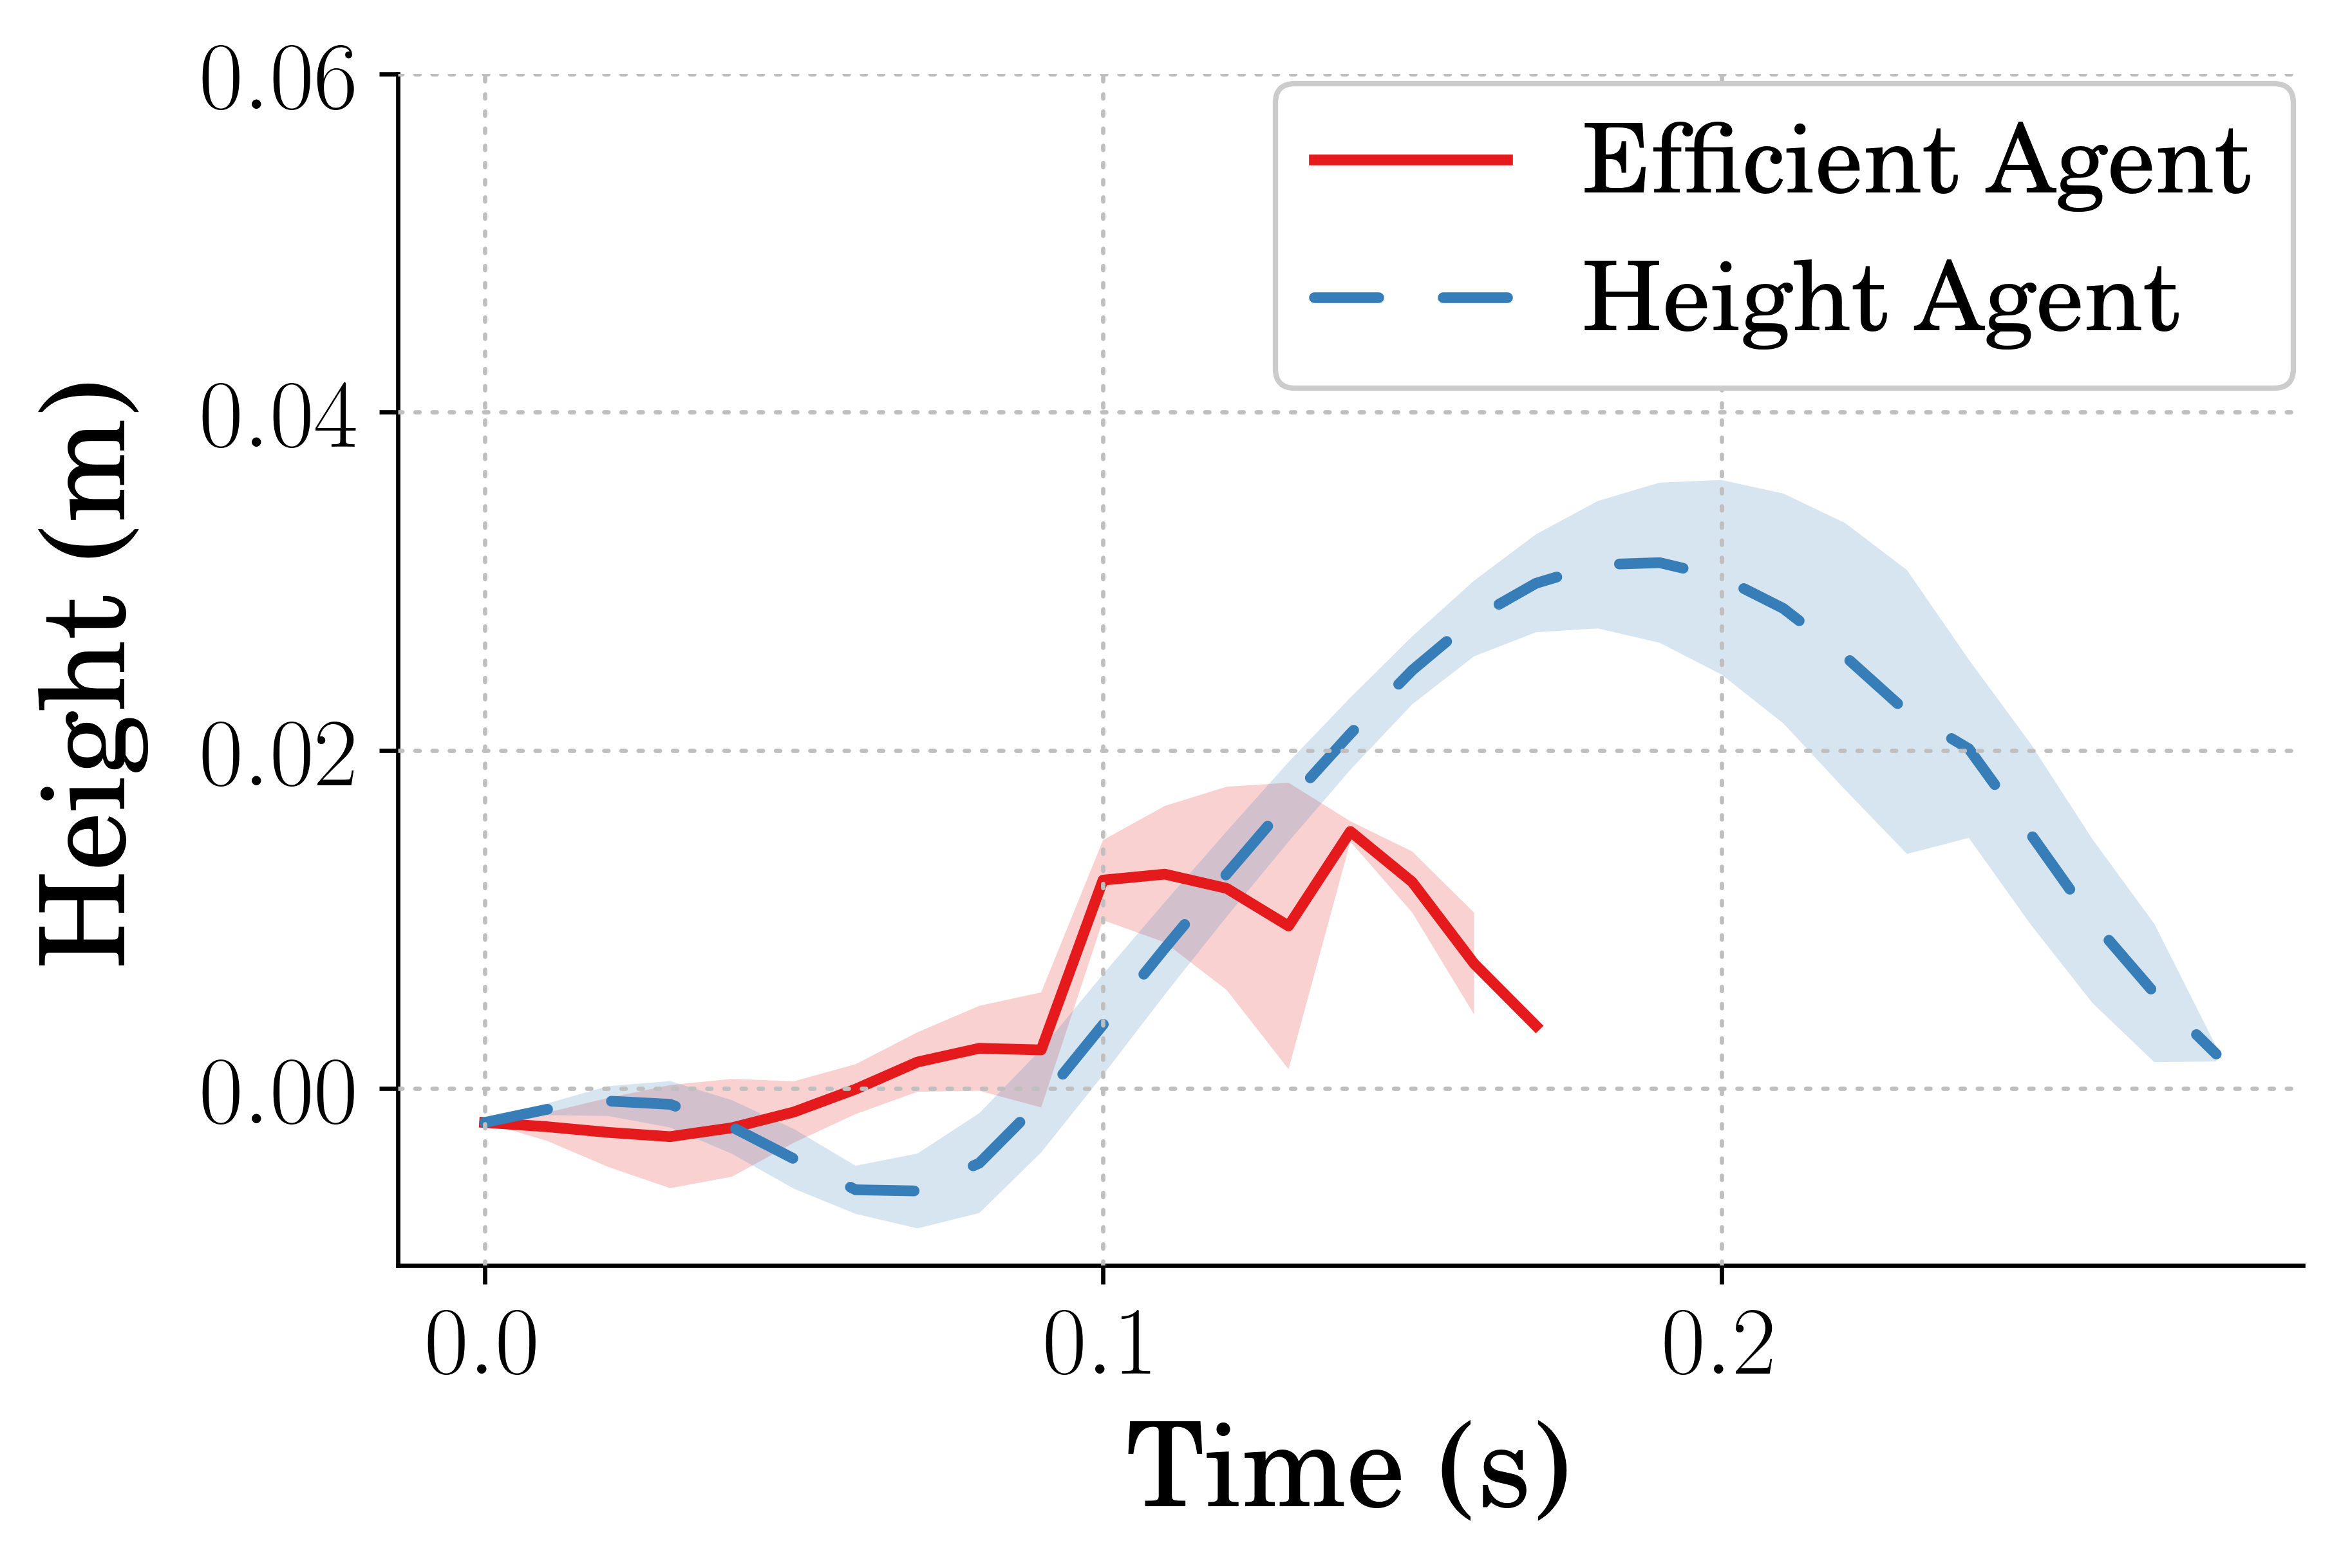
\includegraphics[width=\linewidth]{Figures/Ch2/avg_One_RodPos_.png}
    \caption{Single Jumping Height}
    \label{fig:avg_one_rodpos}
  \end{subfigure}%
  \hfill
  \begin{subfigure}{.49\textwidth}
    \centering
    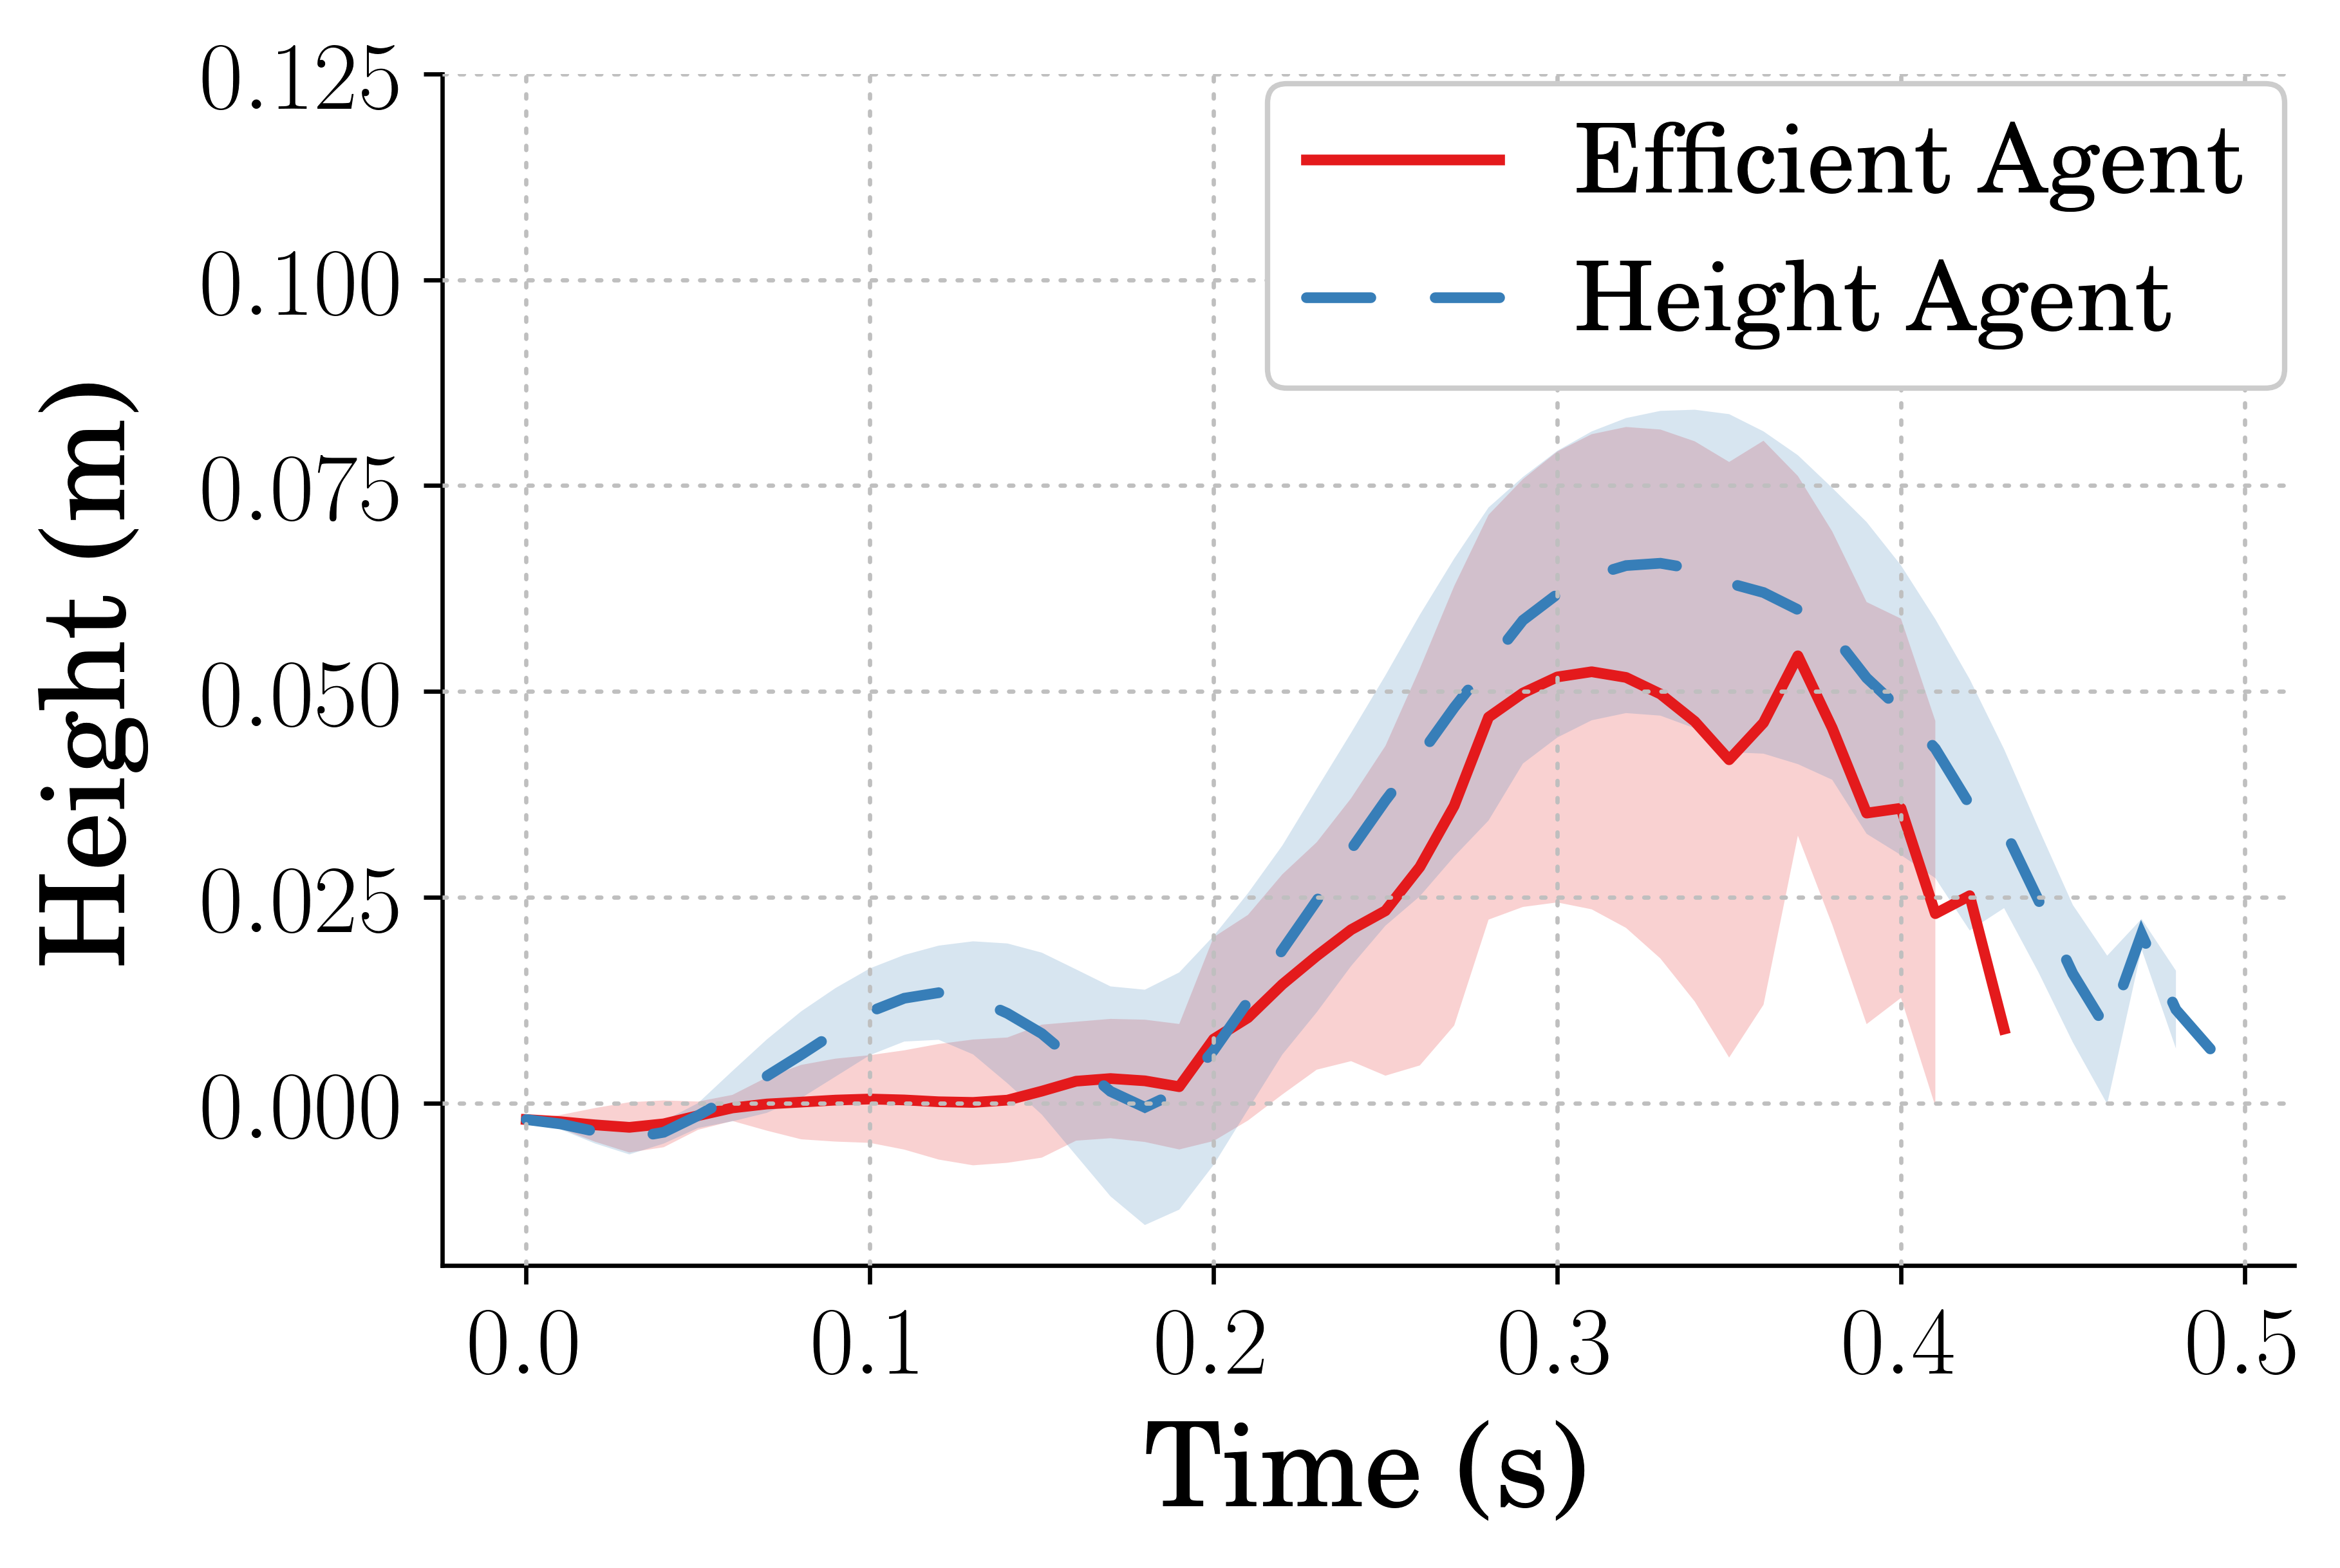
\includegraphics[width=\linewidth]{Figures/Ch2/avg_Stutter_RodPos_.png}
     \caption{Stutter Jumping Height}
     \label{fig:avg_stutter_rodpos}
  \end{subfigure}
   \caption{Average and Standard Deviation Heights of Monopode}
   \label{fig:avg_rodpos}
\end{figure}
% 

The average and standard deviation of the final jumping performance of the controllers are shown in Figure~\ref{fig:avg_rodpos}. In both the single and stutter jumping cases, there are differences in jumping ability when comparing the efficient and height controller types. It is apparent that when increasing the complexity of the command from a single jump to a stutter jump, the efficient controllers are better able to match the performance of the height controllers.

Shown in Figure~\ref{fig:avg_one_rodpos}, the height controllers for the single jumping case learned a command that outperformed the efficient controllers in terms of jump height. The resulting motion from the input discussed in the previous section can be seen in that the efficient controller learned to simply compress the spring, then jump the monopode. The height controllers, in contrast, disregarding power consumption, learned to decompress the spring from its nominal position, keeping it below the point of leaving the ground, then recompressing for a much higher jump. For the single jumping commands, the high-jumping strategy trained controllers that jumped the monopode 104.53\% higher than the efficient-jumping strategy, on average.
% Average Effective Height: 0.01520271583644785
% Average Height Height: 0.031095562970914627
% Percent Difference: 104.53952639412208

Figure~\ref{fig:avg_stutter_rodpos} compares the jumping performance of the efficient and height strategies for the stutter jumping command. They differ, but less drastically than the single jumping case. The similarity of the command shapes shown in Figure~\ref{fig:avg_stutter_input} results in jumping responses that also share a similar form. The large differences seen in the stutter jumping performance are similar to those seen in the inputs, in that they differ mostly regarding the magnitudes. For the stutter jumping command, the high-jumping strategy trained controllers that jumped the monopode 20.69\% higher than the efficient-jumping strategy, on average.
% Average Effective Height: 0.05431672664223123
% Average Height Height: 0.06555982552043371
% Percent Difference: 20.699146604060964

In both the single and stutter jumping cases, the upward acceleration from efficient controllers toward the end of the command can be seen in that the monopode regains height after the start of its final decent from maximum height. This can be explained in that the efficient control method, which punishes power consumption, discovered a way to maintain height throughout a jump where the utilization of additional power is less costly. It is less costly to influence the monopode's position while airborne because there is no resistance from the spring and damper. Additionally, regarding variance, the single jumping controllers seems to produce jumping shapes with similar levels of variance. Whereas in the stutter jumping case, though similar in high levels of input variance, the jumping height variance for the efficient controllers is noticeably higher than that of the height controller. This is likely because the reward for the efficient jumping strategy is fragile, and when learned, is difficult to optimize do to the extreme differences seen in the value received throughout training. A reward that deploys some normalization such that the value returned does not vary greatly would likely result in a better performing final policy.
% 
\subsection{Height reached vs. power used}
\label{subsection:avg_power_used}
% 
\begin{figure}[tb!]
    \centering
    \begin{subfigure}{.49\textwidth}
      \centering
      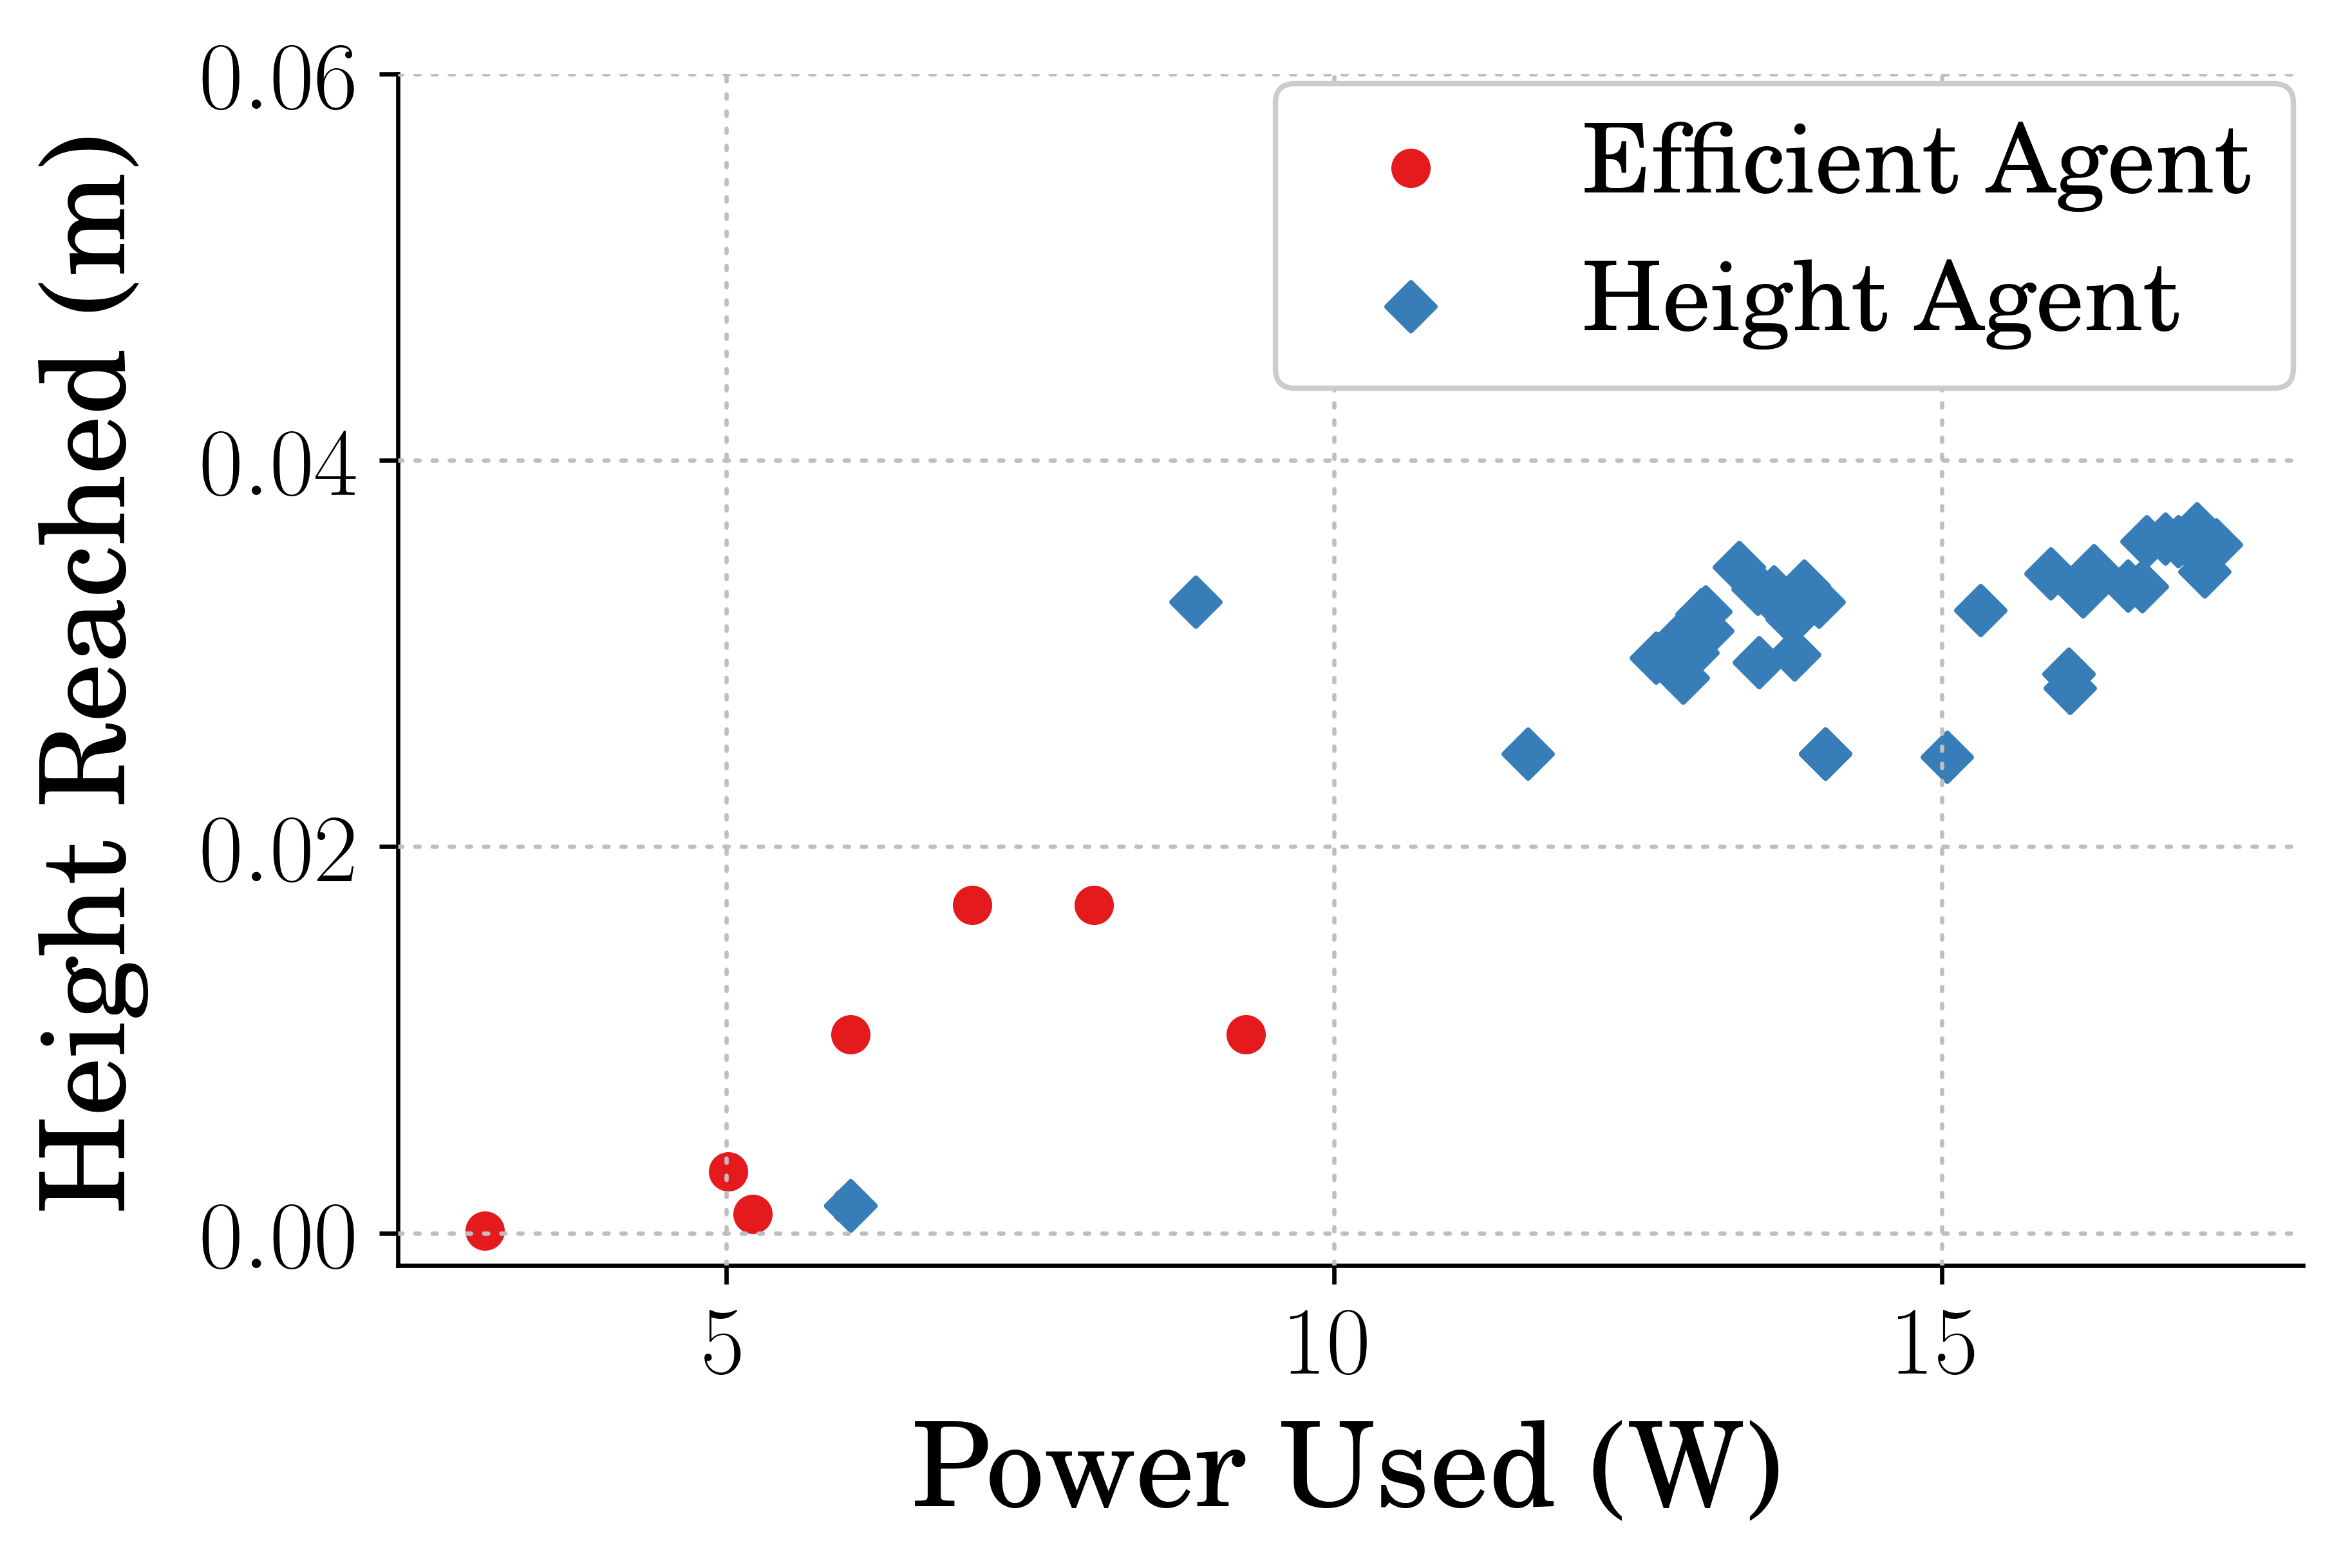
\includegraphics[width=\linewidth]{Figures/Ch2/One_HeightVsPower.png}
      \caption{Single Jumping Efficiency}
      \label{fig:single_heightvspower}
    \end{subfigure}%
    \hfill
    \begin{subfigure}{.49\textwidth}
      \centering
      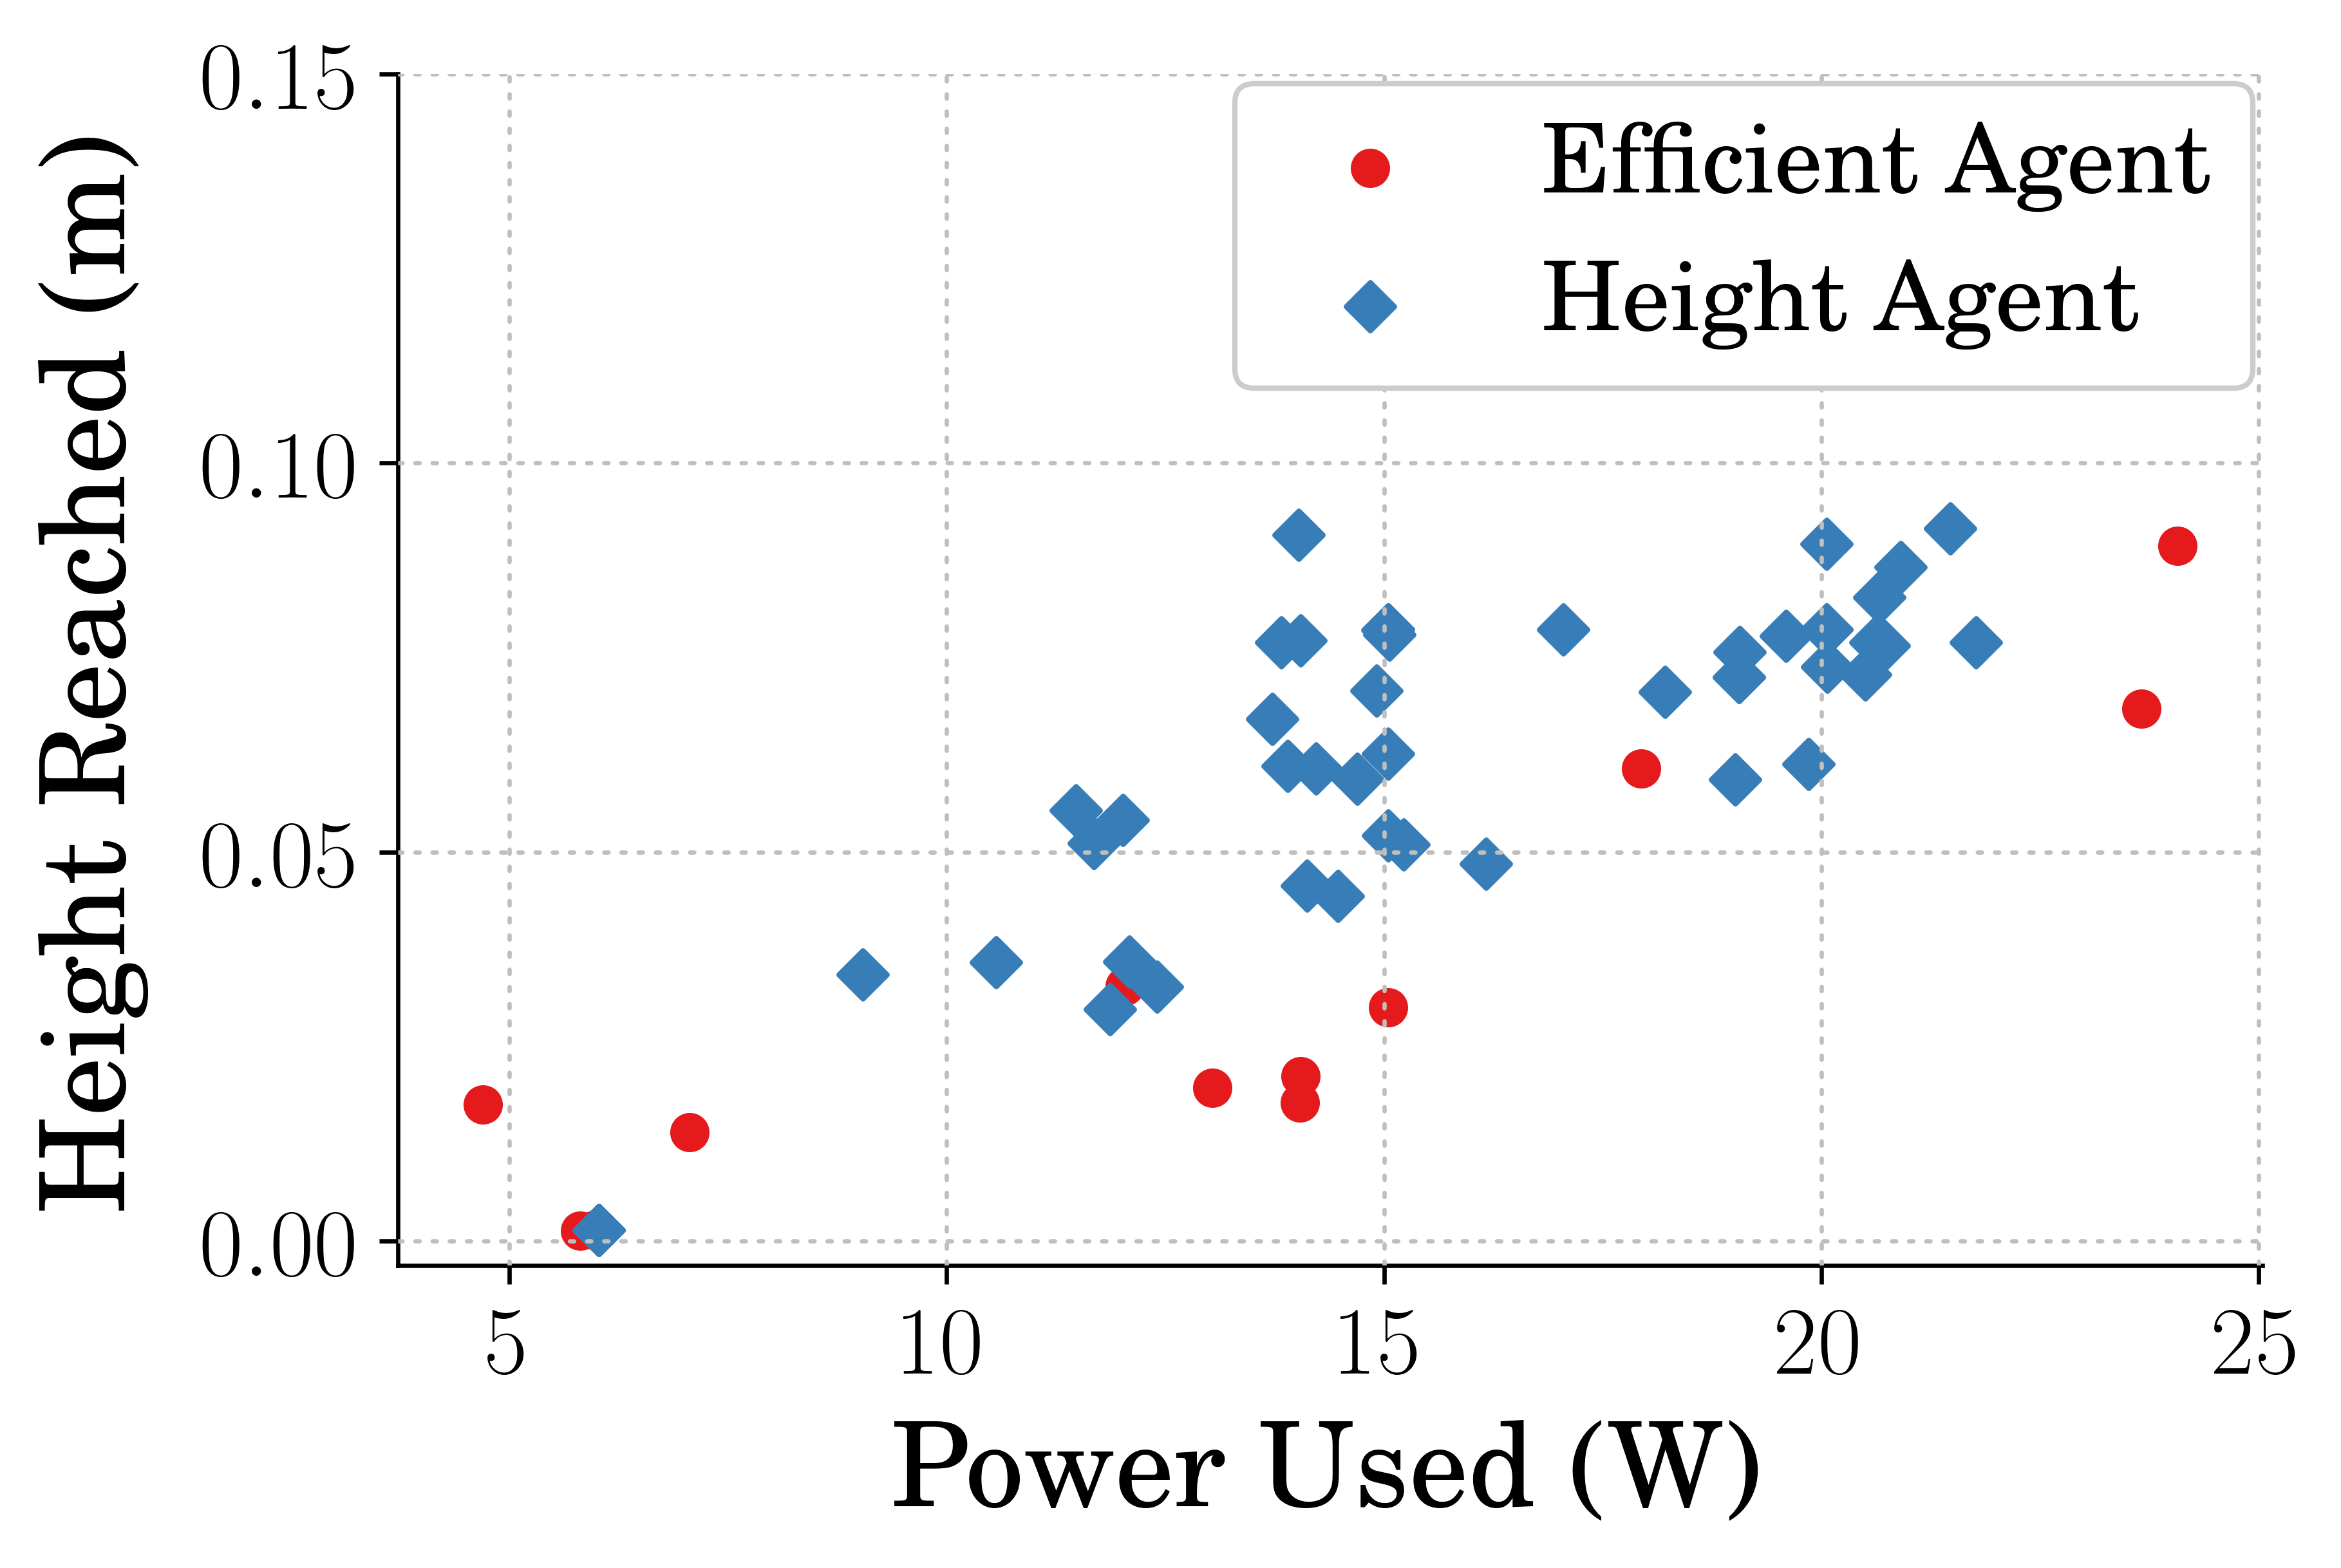
\includegraphics[width=\linewidth]{Figures/Ch2/Stutter_HeightVsPower.png}
       \caption{Stutter Jumping Efficiency}
       \label{fig:stutter_heightvspower}
    \end{subfigure}
     \caption{Height Reached vs Power Consumed of Monopode}
     \label{fig:heightvspower}
\end{figure}
%

The height reached versus power consumed data for both the single jumping and stutter jumping cases, is shown in Figure~\ref{fig:heightvspower}. Although it looks as if there are less efficient instances, this is not the case. The efficient controller types simply learned more consistent control strategies, such that the data points lay on top of one another. This, again, is likely the result of innate fragility within the reward for the efficient controller. Regardless, in both the single and stutter jumping cases, the efficient controllers utilized less power and therefore suffered regarding jump height. This matches what was seen in the previous sections regarding commands and jumping shapes. In both jumping cases, the power conservation gain is greater than the jumping height cost. 

In the single jumping case, shown in Figure~\ref{fig:single_heightvspower}, there is an apparent separation between the two controller types where the height controllers learn control strategies that use more power and jump higher. On average, for the single jumping command type, the efficient-jumping strategy learned jumping commands that were 126.27\% more efficient at the cost of 104.53\% in average jump height.

As for the stutter jumping case, shown in Figure~\ref{fig:stutter_heightvspower}, the difference in performance is less obvious. This can be explained in that more complex jumping strategies give an RL algorithm more opportunity to learn a control policy that can better take advantage of system flexibility. The variance of the two controller types, being quite high, matches what is seen in the previous sections and results in more mixing of the data. On average, for the stutter jumping command type, the efficient strategy learned commands that were 101.45\% more efficient with the average maximum jumping height only being punished by 20.69\%.  
% One
% Average Efficient Power Used: 6.04808059689131
% Average Height Power Used: 13.685329381232417
% Percent Difference: 126.27557887152865
% Stutter
% Average Efficient Power Used: 7.756476293149168
% Average Height Power Used: 15.625778318248924
% Percent Difference: 101.45460035828692 

\section{Optimal Performance of the Proposed Controller}
\label{section:opt_performance}
% 
\subsection{Jumping commands}
\label{subsection:opt_input_performance}
% 
\begin{figure}[tb!]
    \centering
    \begin{subfigure}{.49\textwidth}
      \centering
      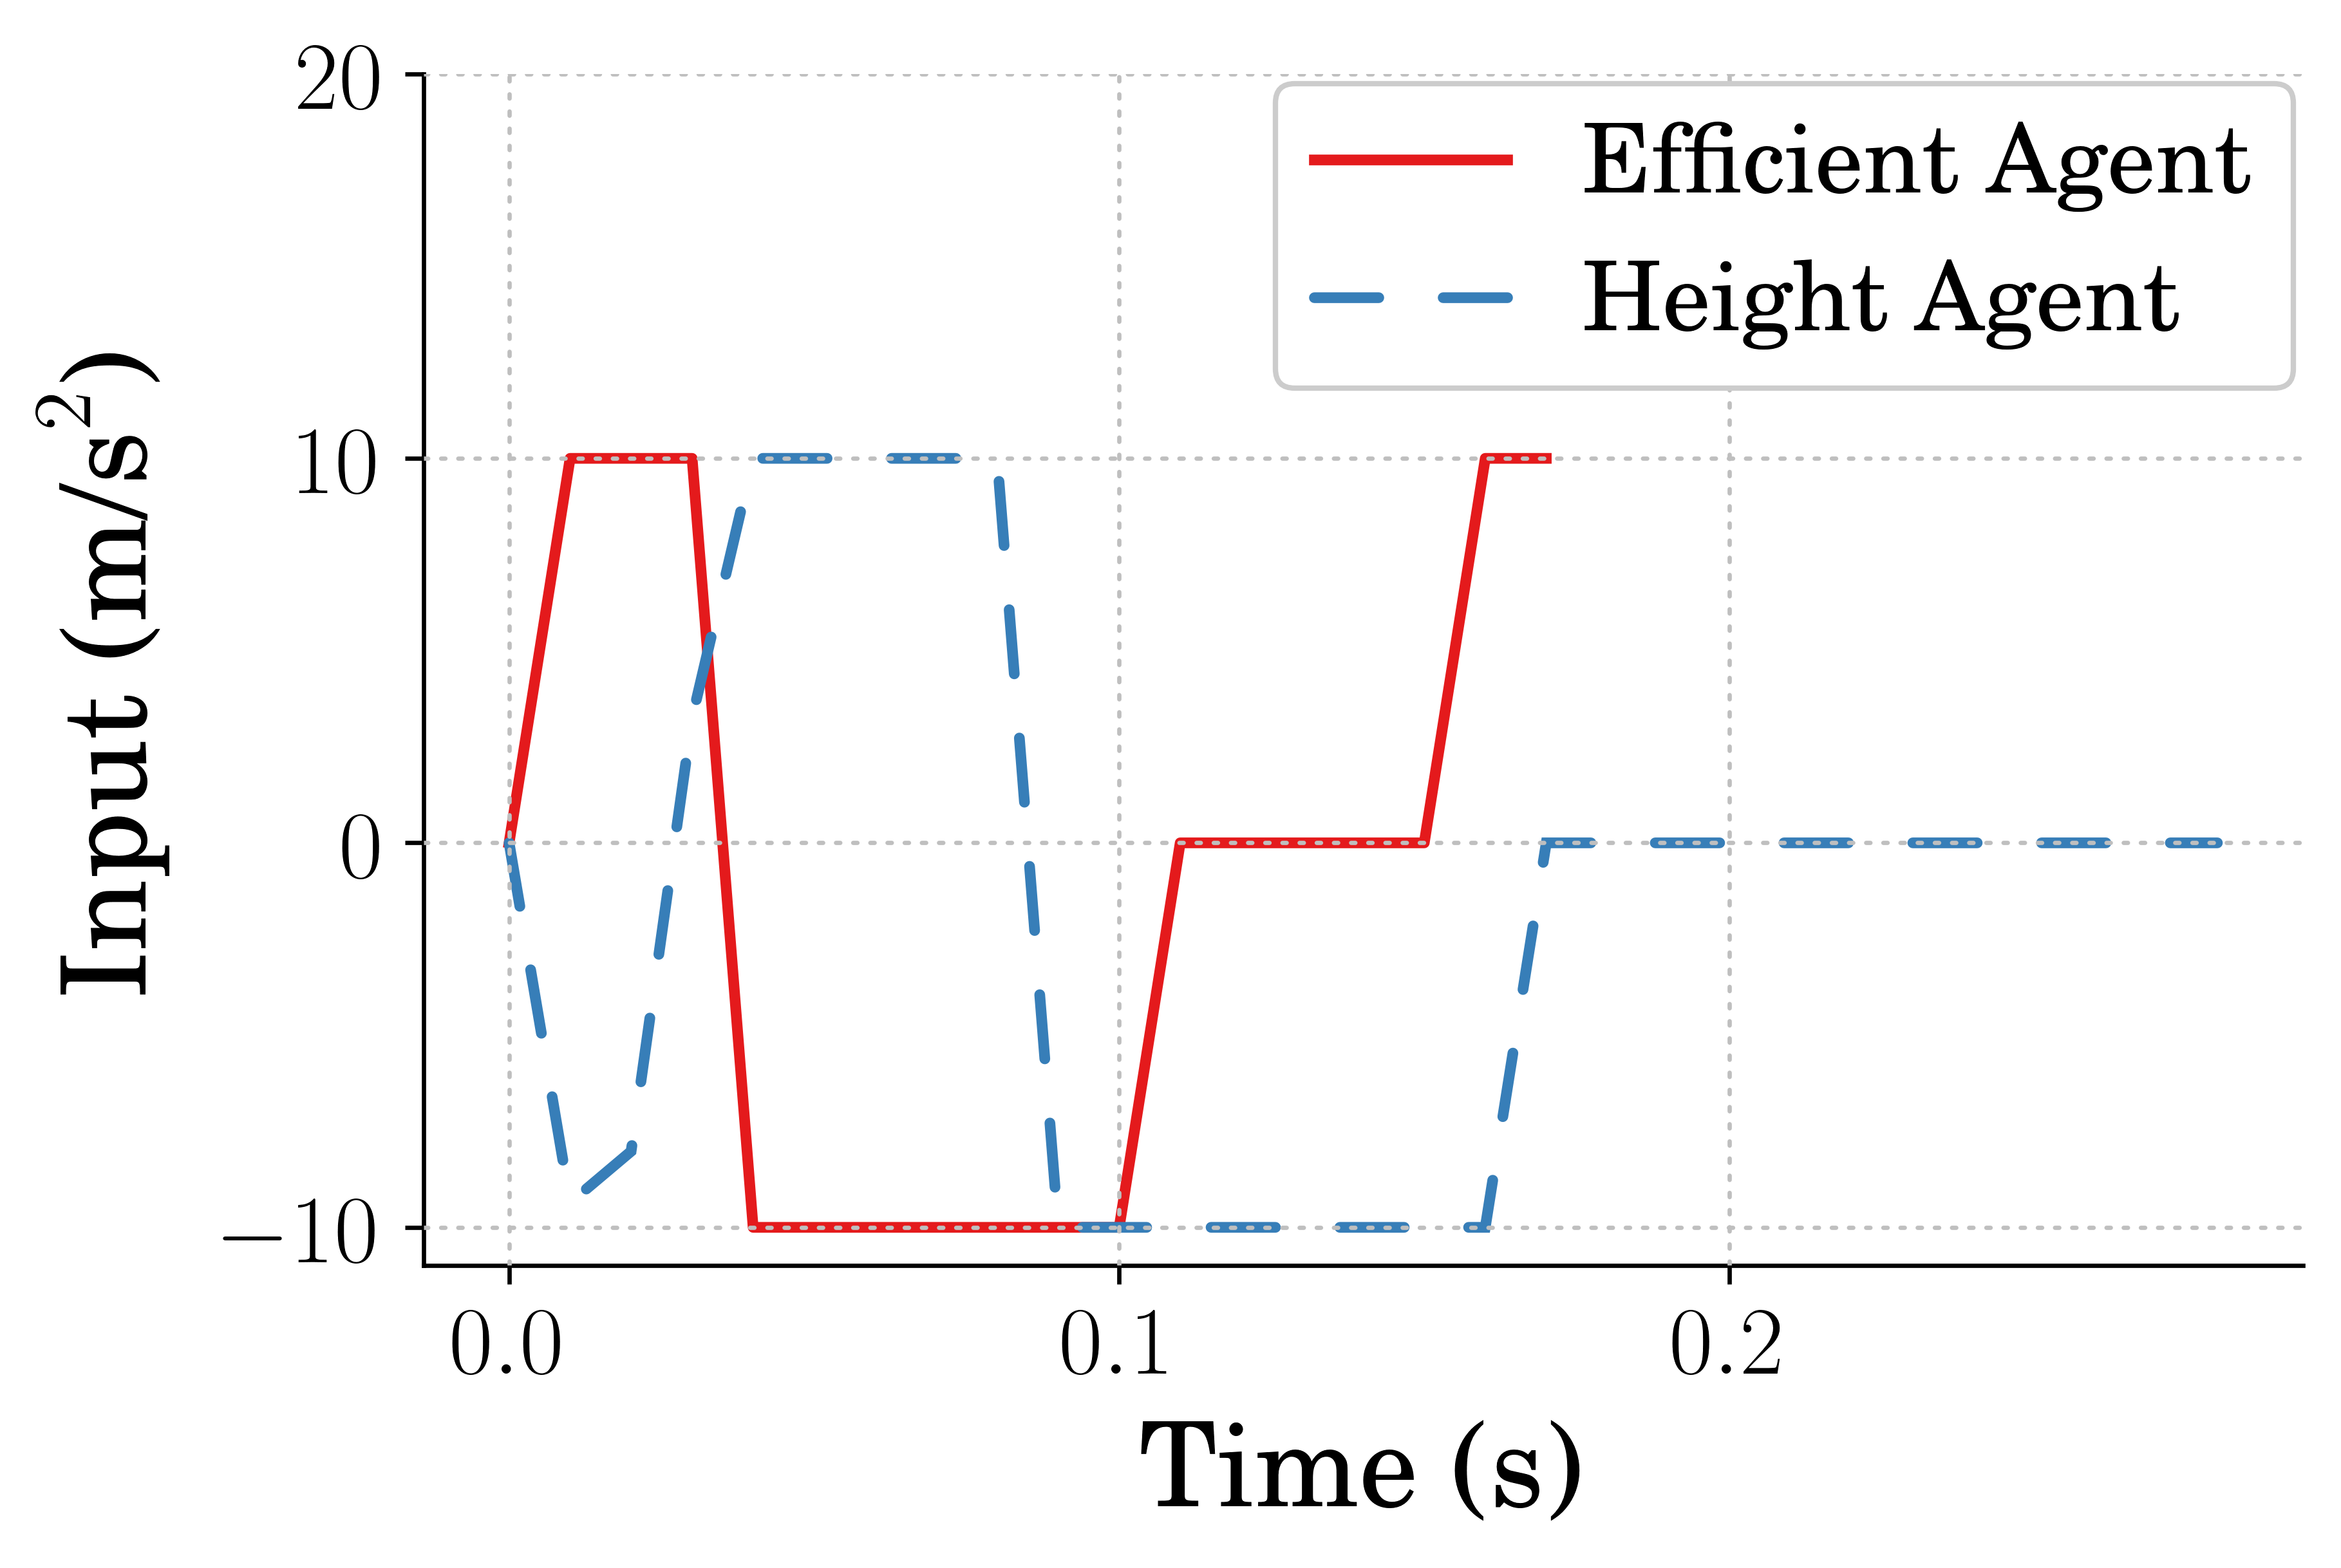
\includegraphics[width=\linewidth]{Figures/Ch2/best_One_Input_.png}
      \caption{Single Jumping Input}
      \label{fig:opt_one_input}
    \end{subfigure}%
    \hfill
    \begin{subfigure}{.49\textwidth}
      \centering
      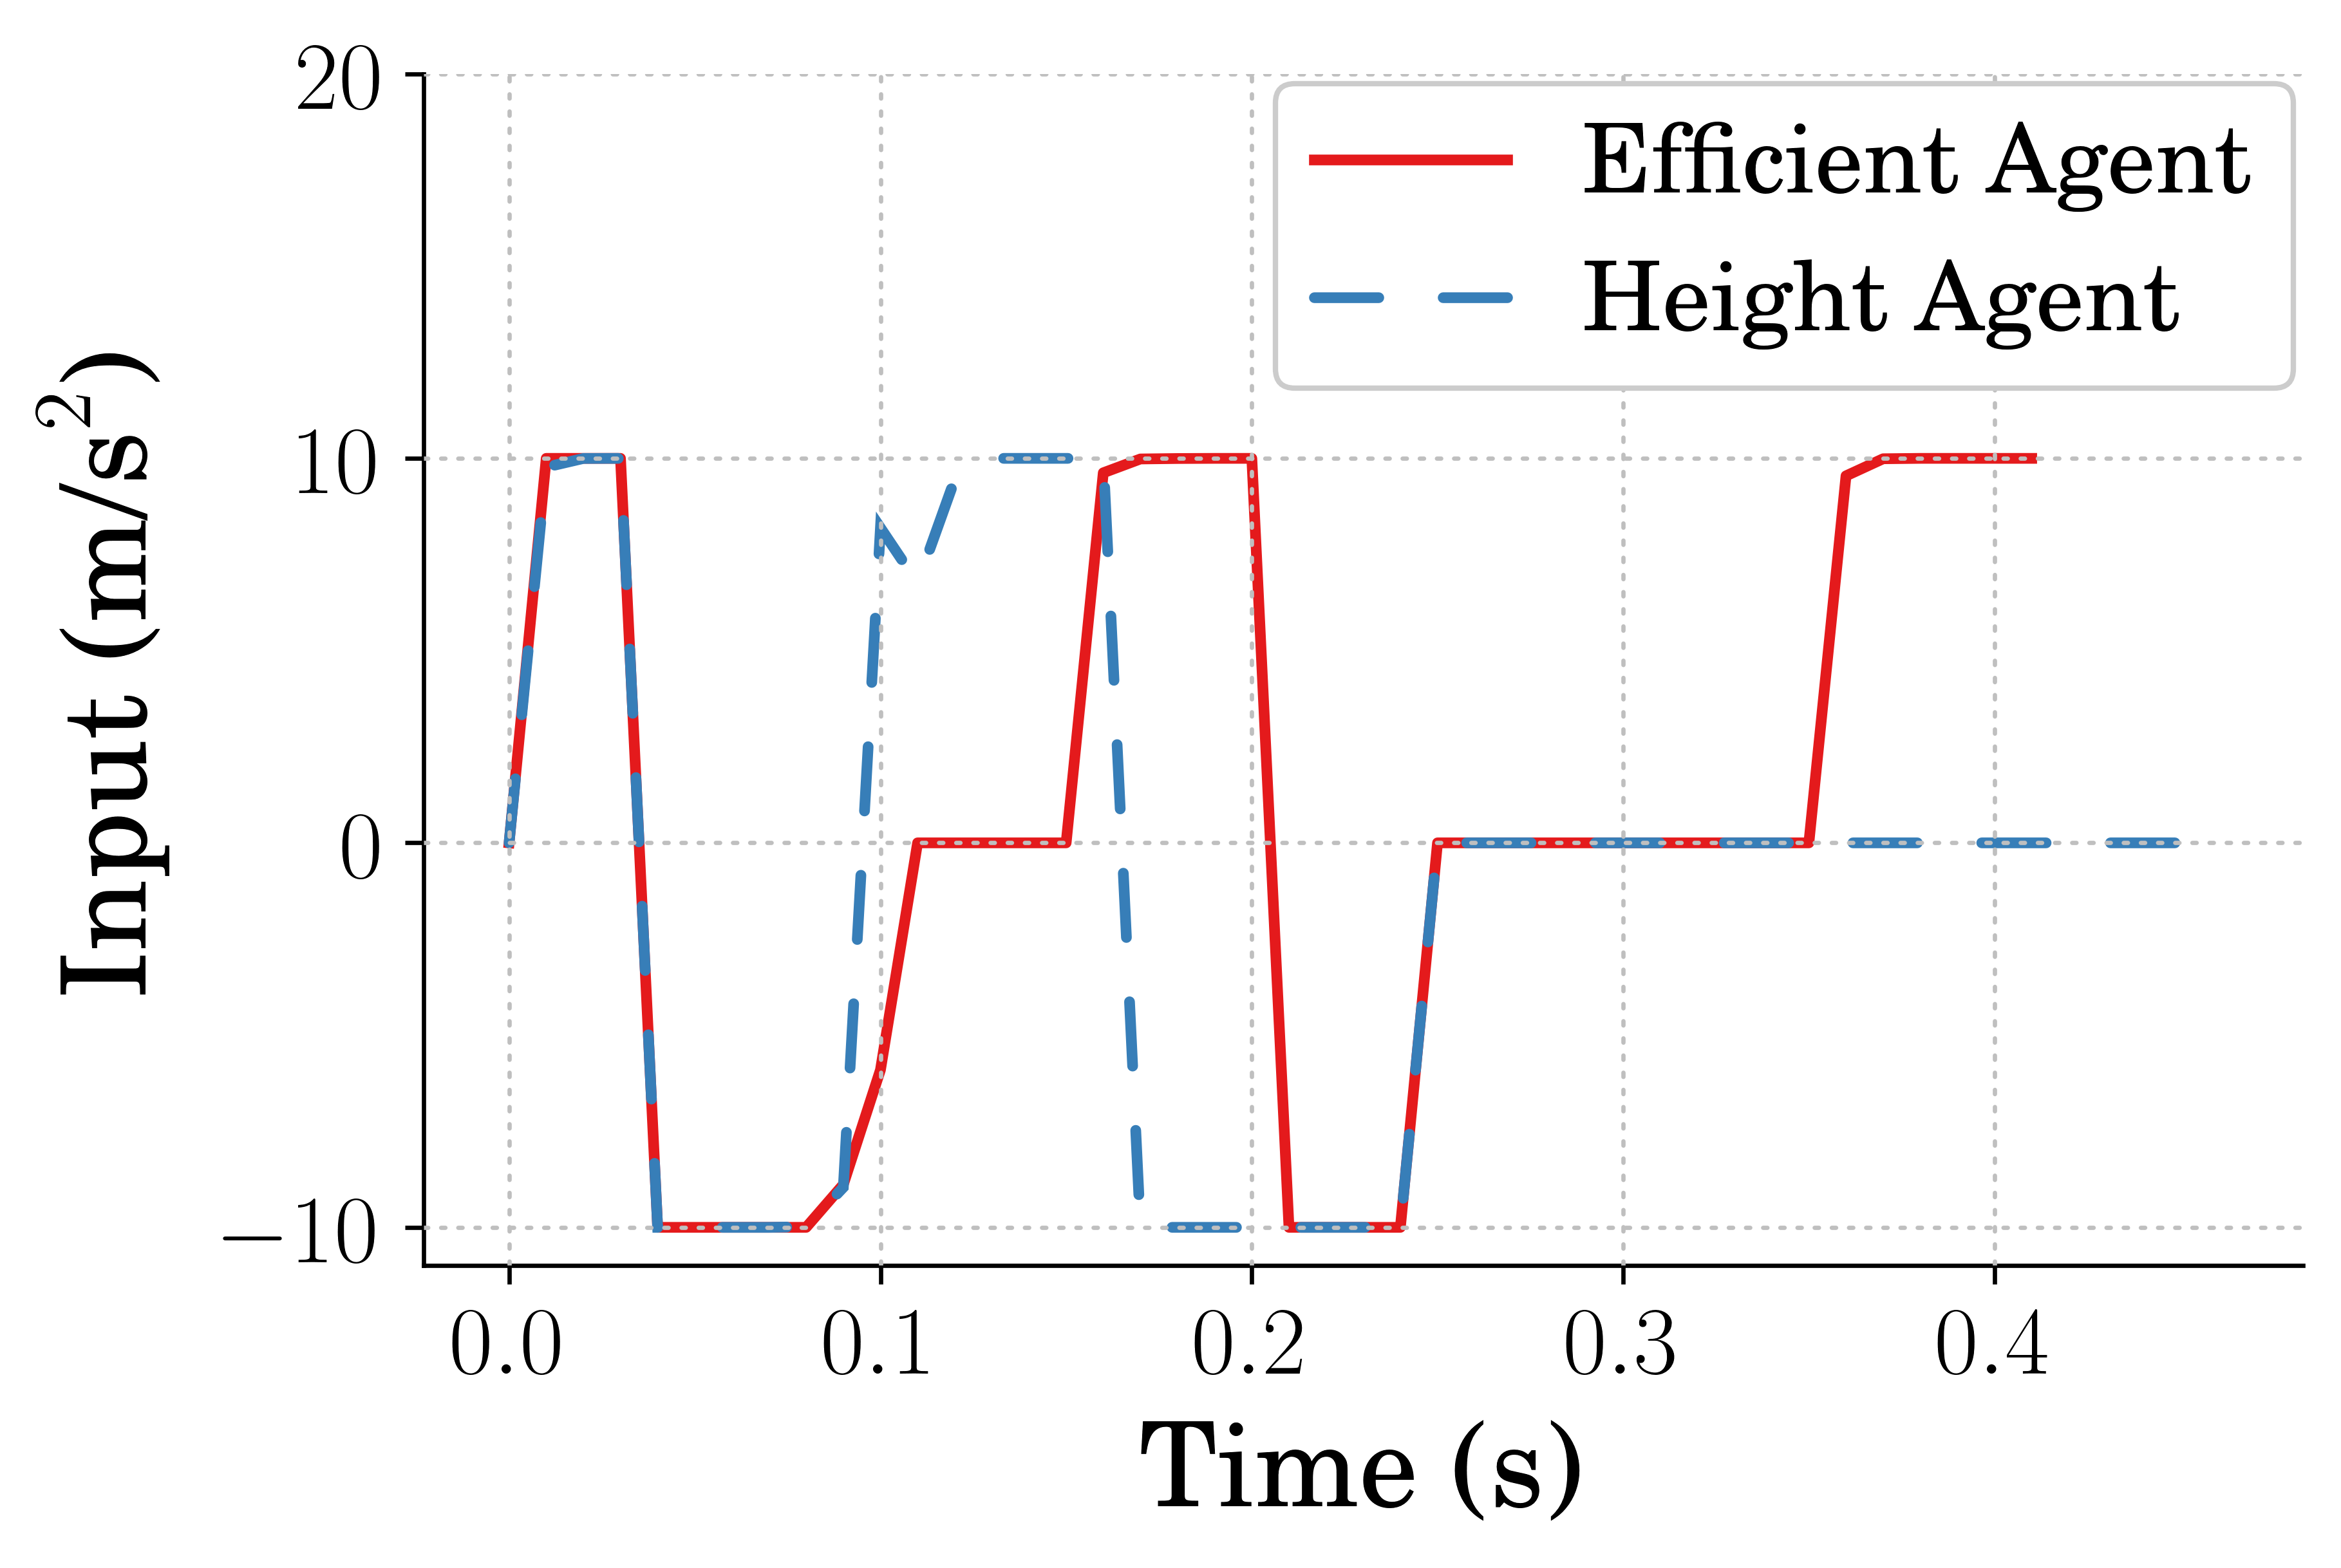
\includegraphics[width=\linewidth]{Figures/Ch2/best_Stutter_Input_.png}
       \caption{Stutter Jumping Input}
       \label{fig:opt_stutter_input}
    \end{subfigure}
     \caption{Optimal Inputs to Monopode}
     \label{fig:opt_input}
\end{figure}
% 

Taking the best of the fifty different controllers trained for both the single and stutter jumping cases and comparing the efficient and height performance of the controllers can show what is possible with a properly defined RL problem. Figure~\ref{fig:opt_input} shows the differences in the commands generated when selecting the highest performing controller in terms of reward received. It can be seen that there are less differences between the efficient and height controllers in comparison to the average results from Section~\ref{section:avg_performance}. A major similarity is that magnitudes are similar across all cases such that the controllers utilize the maximum acceleration of the actuator. 

Looking at Figure~\ref{fig:opt_one_input}, which compares the efficient and height controllers for the single jumping input, the major differences are the timing and direction of the commands. This is similar to the average performance evaluation, from Section~\ref{subsection:avg_input_performance}, in that the efficient controller does not take advantage of the slight decompression of the spring before the monopode leaves the ground. Because of this, the efficient controller learns a different timing for a single jump. 

As for the stutter jumping case, shown in Figure~\ref{fig:opt_stutter_input}, the differences between the efficient and height controller are less drastic. The initial timing is largely the same as both controller types learn to utilize the decompression of the spring. The differences begin when decompressing the spring a second time and completing the first jump. The efficient controller learns a command similar in form to a bang-coast-bang command, where, in contrast, the height controller learns a command similar to that of a bang-bang shaped input. Bang-bang based commands have been shown to generate optimal jumping performance for high jumps for the monopode jumping system \cite{Vaughan2013}. Additionally bang-coast-bang shaped commands have been shown to be ones which could increase power efficiency \cite{doi:10.2514/2.4036}
% 
\subsection{Jumping height performance}
\label{subsection:opt_height_performance}
% 
\begin{figure}[tb!]
    \centering
    \begin{subfigure}{.49\textwidth}
      \centering
      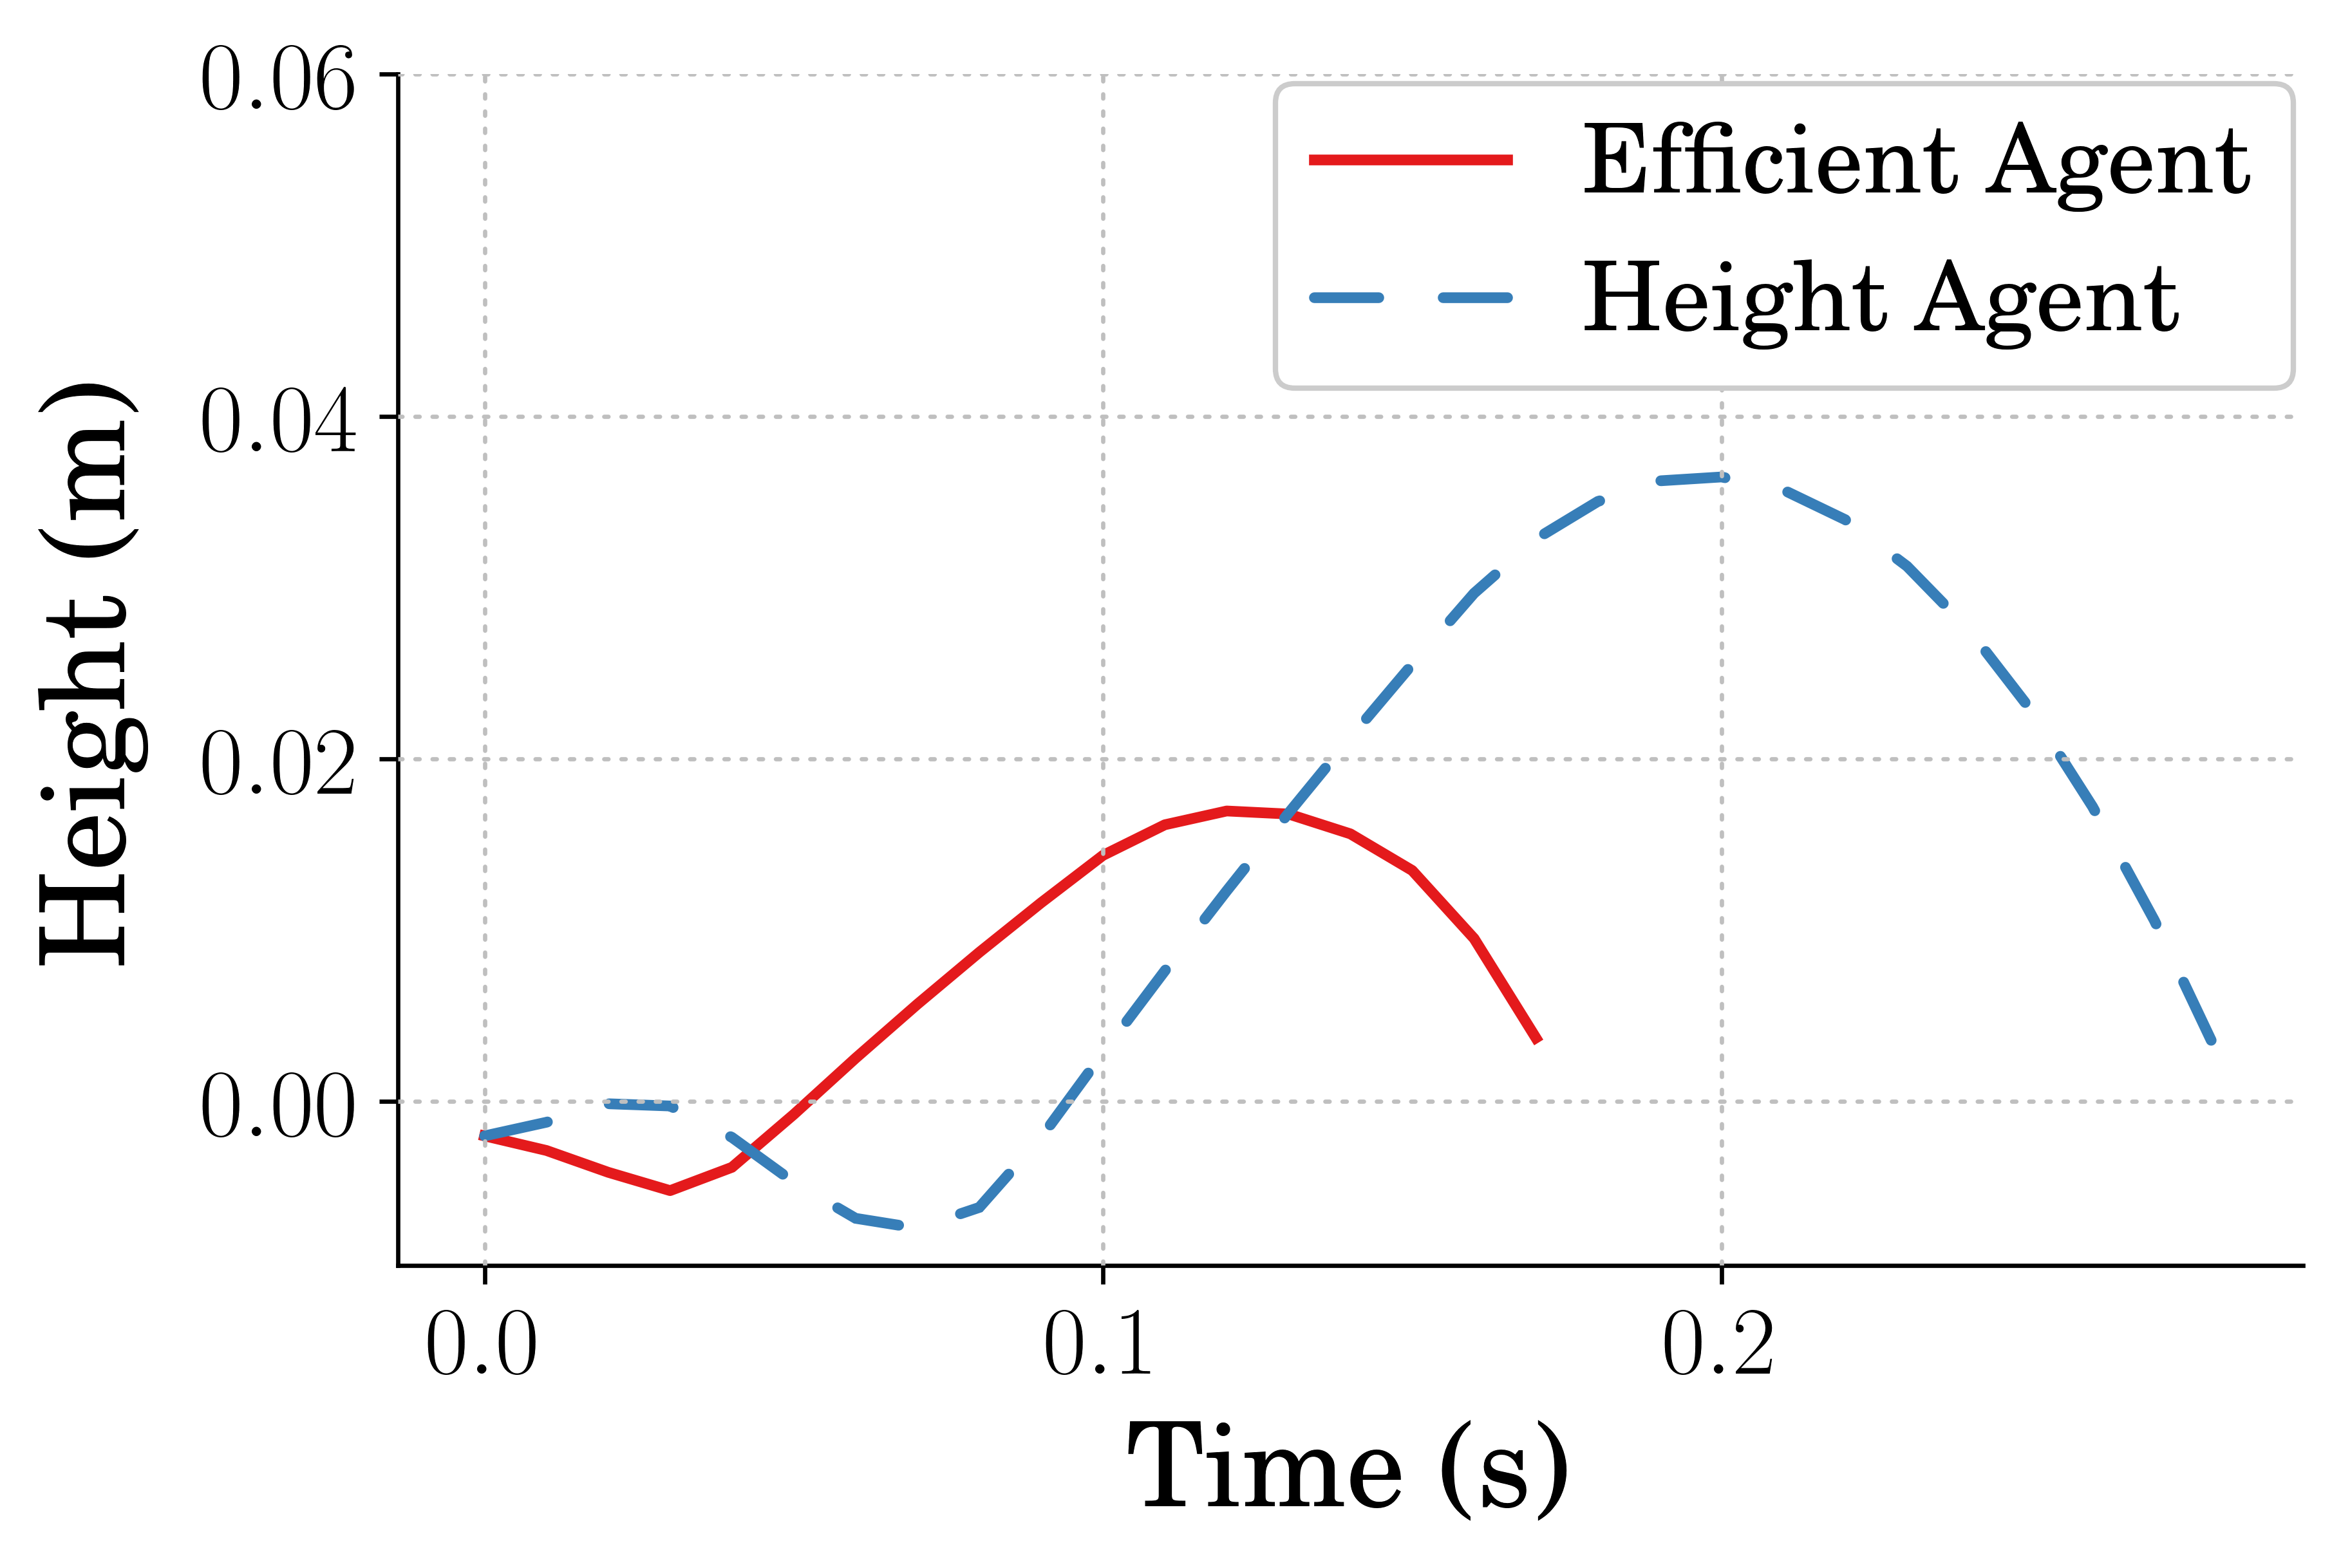
\includegraphics[width=\linewidth]{Figures/Ch2/best_One_RodPos_.png}
      \caption{Single Jumping Height}
      \label{fig:opt_one_rodpos}
    \end{subfigure}%
    \hfill
    \begin{subfigure}{.49\textwidth}
      \centering
      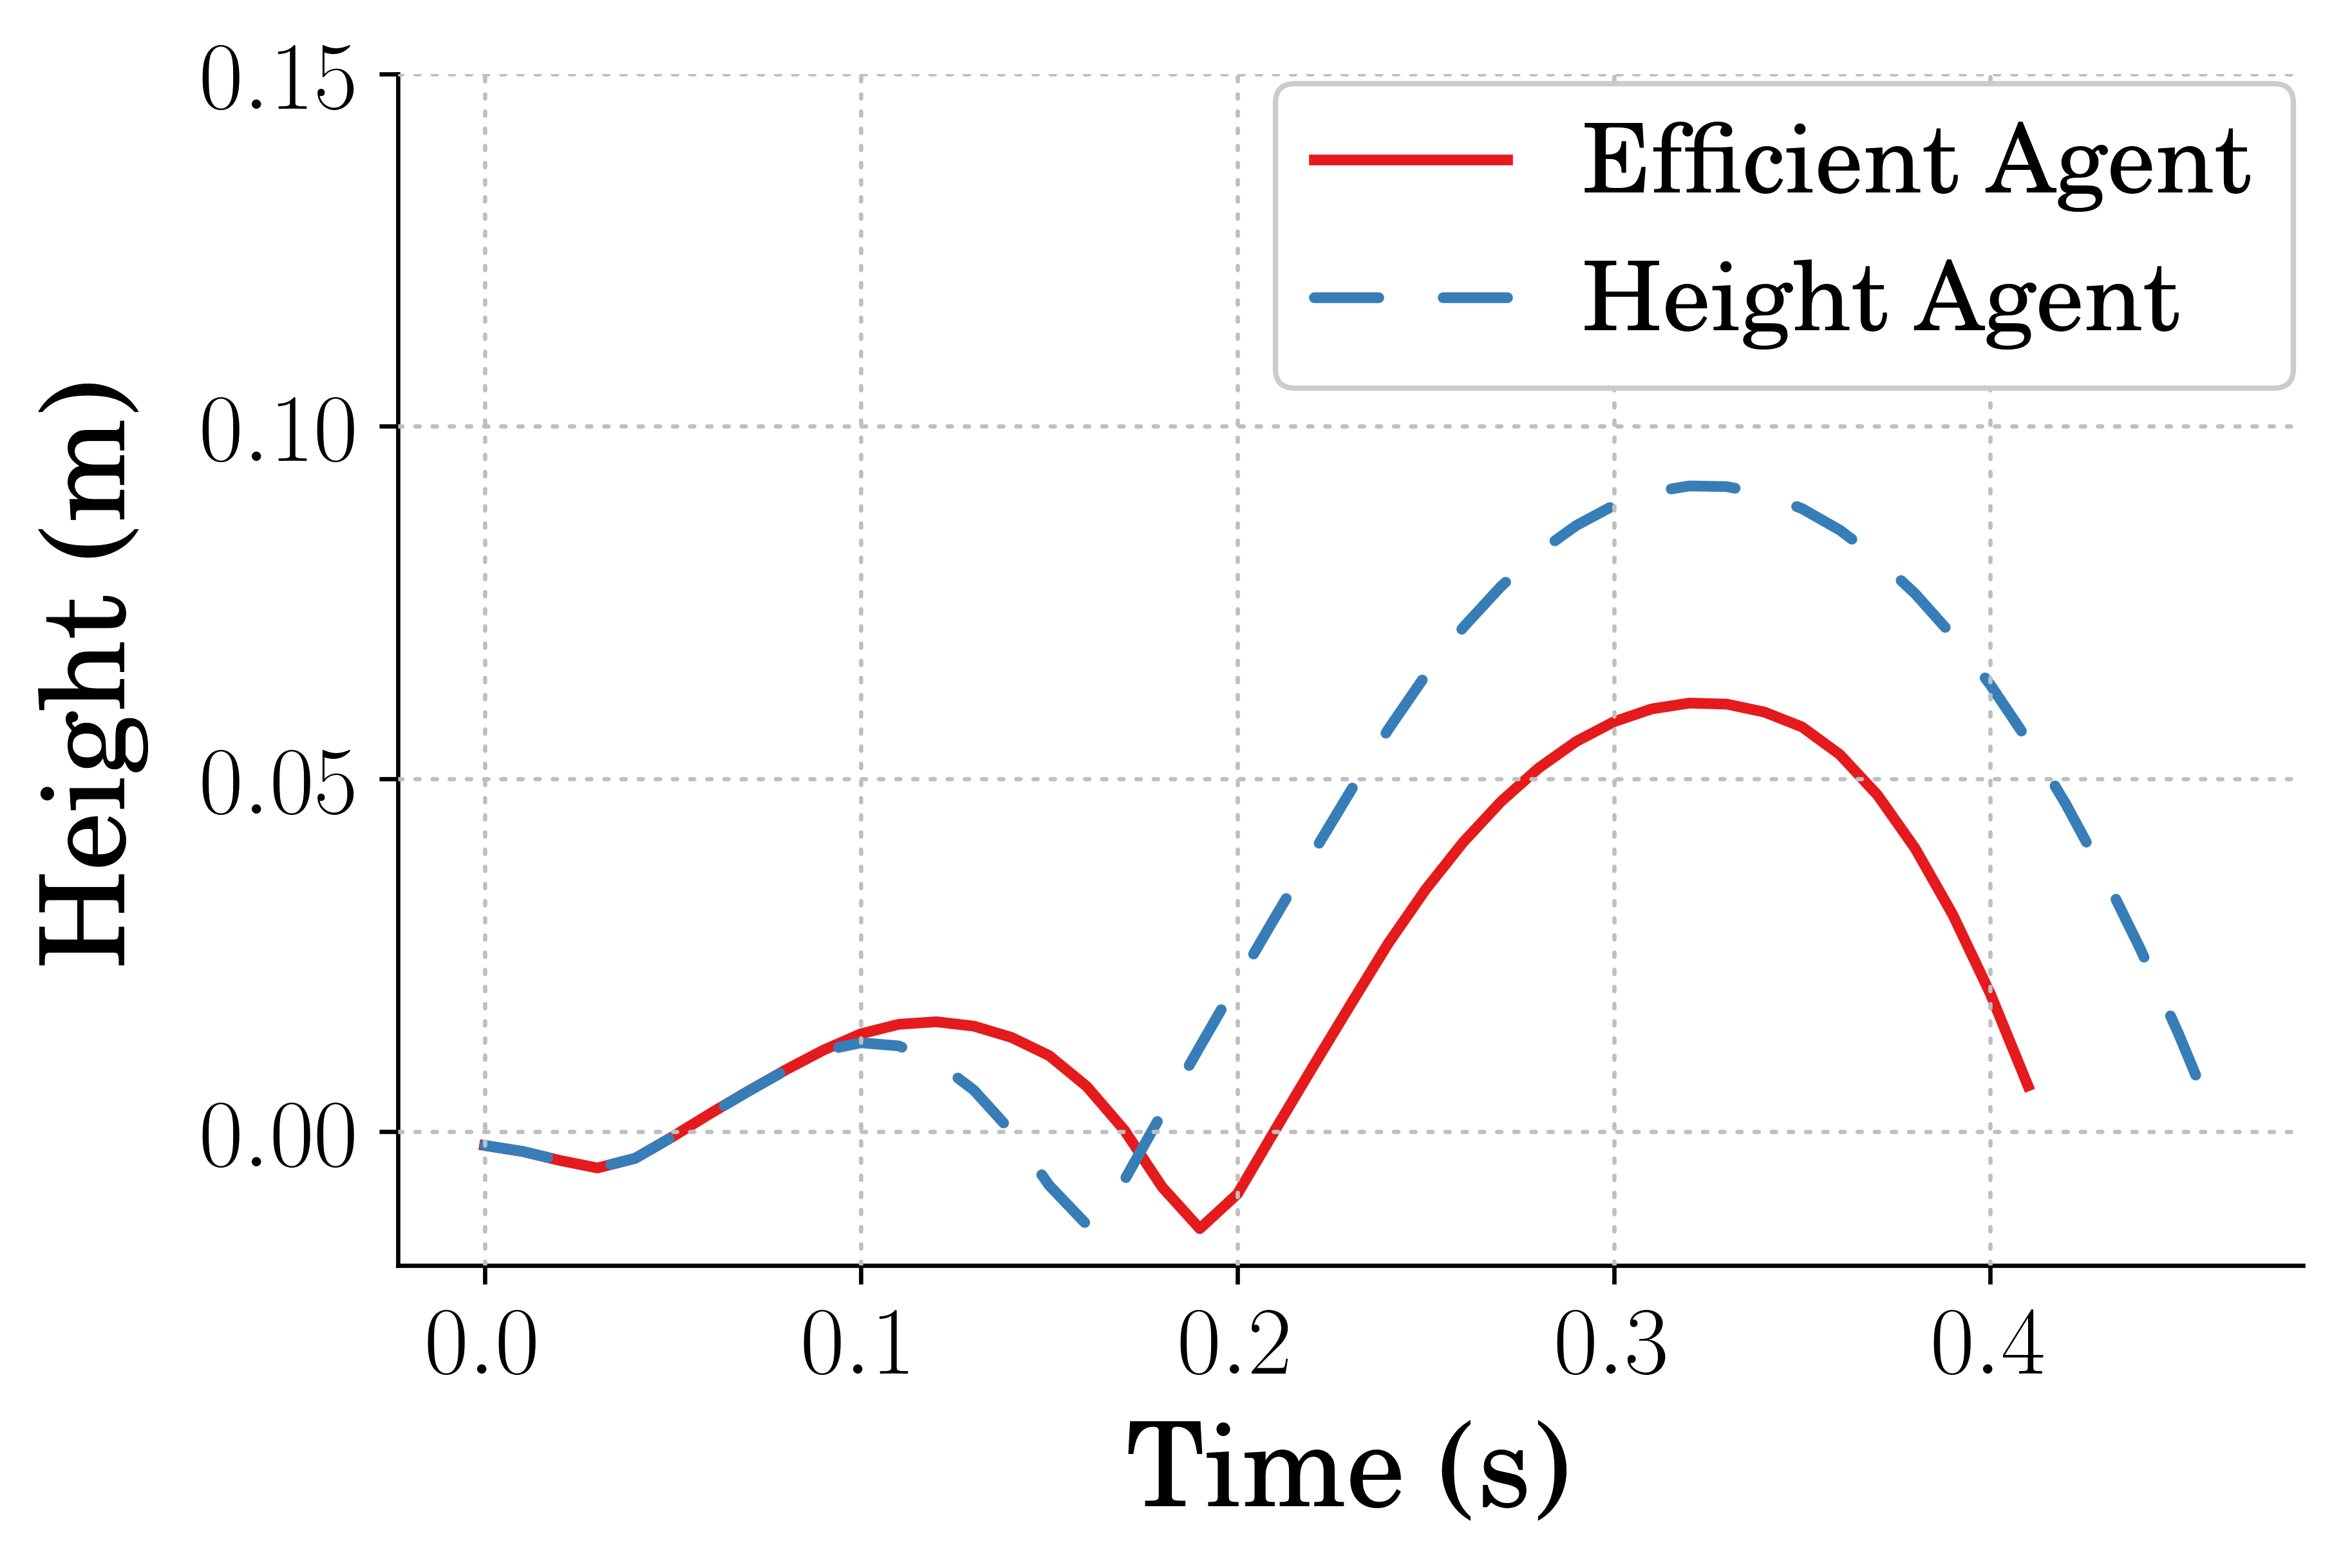
\includegraphics[width=\linewidth]{Figures/Ch2/best_Stutter_RodPos_.png}
       \caption{Stutter Jumping Height}
       \label{fig:opt_stutter_rodpos}
    \end{subfigure}
     \caption{Optimal Heights of Monopode}
     \label{fig:opt_rodpos}
\end{figure}
% 

Figure~\ref{fig:opt_rodpos} displays the jumping performance for both jump types as well as both controller types when utilizing the inputs shown in Section~\ref{subsection:opt_input_performance}. These curves show that the efficient controllers, in the best case scenario, do not generate commands that jump the monopode as high as the high jumping controllers.

Figure~\ref{fig:opt_one_rodpos}, which compares the efficient and height controllers for the single jump, shows that the efficient controller does not learn to utilize the allowable decompression in the spring. In Figure~\ref{fig:opt_stutter_rodpos}, it can be seen that when utilizing a command more similar in form to a bang-coast-bang command, like the efficient controller learned, the timing of the jump sequence is shifted and the resulting final height is less than the height controller where the command is more similar to a bang-bang shaped command. The efficient controller having learned to coast between commands shows it is a useful method for conserving power, but not a good strategy for optimizing jumping height. 
% One
% Max Efficient Height: 0.0169633024040252
% Max Height Height: 0.0364650959908489
% Percent Difference: 114.96460490025893
% Max Efficient Power Used: 8.023999999999997
% Max Height Power Used: 17.101847234287263
% Percent Difference: 113.13368936050934
% Stutter
% Max Efficient Height: 0.0607432013800848
% Max Height Height: 0.0915456169114579
% Percent Difference: 50.70923960466784
% Max Efficient Power Used: 17.93805315775764
% Max Height Power Used: 21.476888231927703
% Percent Difference: 19.72808890155189

\section{Conclusion}
Two different controller types were trained to generate two different jumping commands for the simplified monopode jumping system. The first type of controller was one that would command the monopode system to jump high where the reward was based on nothing other than system height. The second type of controller was one which controlled the monopode to jump high but at the cost of power consumed, such that high jumps that consumed high amount of power were less desirable than high jumps that consumed less power. It was shown that the rewards passed to RL algorithms that are training controllers can be manipulated so that the learned commands take advantage of the spring/damper that exists within the monopode jumping system. Furthermore, the timing of the commands, as well as the input magnitude and direction are all affected when defining a reward strategy that seeks to increase power efficiency. When considering the average performance of the different control strategies, for both the single and stutter jumping cases, the heights reached were less for the efficient strategies. However, they were significantly more efficient, particularly when scaling the complexity of the command from the single jump to the stutter jump. It should then be concluded that RL might serve as a useful method for defining control strategies for flexible-legged jumping systems, particularly when energy efficiency is of interest. Additionally, when considering more complex control strategies, which might be difficult to define efficiently, RL might serve as a useful method for effective efficient strategies.